% AER-Article.tex for AEA last revised 22 June 2011
\documentclass[pdftex]{article}

\RequirePackage[OT1]{fontenc}

\RequirePackage{graphicx}
\RequirePackage{amsthm}
%\RequirePackage{amsmath}
\RequirePackage{natbib}
%\RequirePackage[colorlinks,citecolor=blue,urlcolor=blue]{hyperref}
%\RequirePackage{hypernat}
\RequirePackage[dvips]{color}
%\RequirePackage{breqn}
%\Requirepackage[T1]{fontenc}
\RequirePackage[latin9]{inputenc}
%\RequirePackage{enumitem}
%\RequirePackage{bbm}
\RequirePackage{amssymb}
\RequirePackage{stmaryrd}
\RequirePackage{nicefrac}
%\RequirePackage{amsfonts}
%\RequirePackage[english]{babel}
\RequirePackage{tikz}

%\RequirePackage[OT1]{fontenc}
%\RequirePackage{graphicx}
%\RequirePackage{amsthm}
\RequirePackage[cmex10]{amsmath}
%\RequirePackage{natbib}
%\RequirePackage[colorlinks,citecolor=blue,urlcolor=blue]{hyperref}
%\RequirePackage{hypernat}
\RequirePackage[dvips]{color}
%\RequirePackage{breqn}
%\Requirepackage[T1]{fontenc}
%\RequirePackage[latin9]{inputenc}
\RequirePackage{enumitem}
\RequirePackage{bbm}
%\RequirePackage{amssymb}
%\RequirePackage{stmaryrd}
%\RequirePackage{nicefrac}
\RequirePackage{amsfonts}
%\RequirePackage[english]{babel}
%\RequirePackage{tikz}
\usepackage{subcaption}
\usepackage{setspace}
\usepackage{caption}
\usepackage{authblk}
%\startlocaldefs



\numberwithin{equation}{section}
\newtheoremstyle{th}
  {\topsep}%Space above
  {\topsep}%Space below
  {\itshape}%Body font
  {}%Indent amount
  {\normalfont}% Theorem head font
  {:}%Punctuation after theorem head
  { }%Space after theorem head
  {}% Theorem head specification
\theoremstyle{th}
\newtheorem{thm}{{Theorem}}%[section]
\newtheorem{lemma}{{Lemma}.}%[section]
\newtheorem{conjecture}{{Conjecture}.}%[section]
\newtheorem{prop}{{Proposition}}%[section]
  \newtheorem{cor}{{Corollary}}%[section]%{\protect\corollaryname}
\newtheorem{proof lemma}{{Proof Lemma}.}
\theoremstyle{definition}
\newtheorem{A}{A\hspace{-0.15cm}}
\newtheorem{B}{B\hspace{-0.15cm}}
\newtheorem*{TK}{TK\hspace{-0.15cm}}
\newtheorem*{JS}{JS\hspace{-0.15cm}}
\newtheorem{SA}{SA\hspace{-0.15cm}}
\newtheorem{ceu}{CEU\hspace{-0.15cm}}
\newtheorem{definition}{Definition}%[section]
\newtheorem{example}{Example}%[section]
\newtheorem{remark}{Remark}%[section]
\newtheorem{statement}{Statement.}%[section]
\newtheorem{fact}{Fact}%[section]
\newtheorem*{risk lovers}{Risk lovers}
\newtheorem*{risk averse}{Risk averse}


%\Spacing{2}

\begin{document}

\title{General Equilibrium with Risk Loving, Friedman-Savage and other Preferences}
\author[1,2]{A. Araujo\thanks{We thank participants at the 10th Annual Cowles GE 2014 Conference, the 13th SAET 2013 Conference, EEA-ESEM 2014, IWGTS 2014, EWGET 2014, LACEA-LAMES 2014, the 15th SAET 2015 Conference and the 11th World Congress of the Econometric Society for comments. We also thank T. Kehoe, P.A. Chiappori, P. Wakker, T. Strzalecki and C. Azariadis for their comments and suggestions that improved our work. The authors gratefully acknowledge financial support from CAPES, CNPq and FAPERJ, Chateauneuf and Gama thank IMPA for the generous financial support from the ``Ci\^{e}ncias sem Fronteiras'' fellowship and from the ``Brazilian$-$French Network in Mathematics''.}\thanks{aloisio@impa.br}}
\author[3]{A. Chateauneuf\thanks{Alain.Chateauneuf@univ-paris1.fr}}
\author[1]{J. Gama\thanks{jpgamat@impa.br}}
\author[4]{R. Novinski\thanks{rodrigo.novinski@ibmecrj.br}}
\affil[1]{IMPA, Rio de Janeiro, Brazil}
\affil[2]{EPGE/FGV, Rio de Janeiro, Brazil}
\affil[3]{IPAG Business School and Paris School of Economics, Universit\'{e} de Paris I, Paris, France}
\affil[4]{Faculdades Ibmec-RJ, Rio de Janeiro, Brazil}

\date{\today}
\maketitle
\vspace{-1cm}
\begin{abstract}
%More and more economists find both empirical and experimental evidence that the economic behavior is well beyond of what it was originally taught. In this paper, we try to reconcile this evidence with the classical economics. In particular, the presence of Risk Lover (or ambiguity lovers, Friedman-Savage and related behavior) have not yet been extensively analyzed in the general equilibrium literature due to lack of convexity and{, hence, failure of} existence.

More and more economists find both empirical and experimental evidence of economic behavior that is well beyond classical economics. In particular, the empirical evidence (\cite{JS}), and the experimental evidence (\cite{KT} and the one found in \cite{Wakker}) supported the importance of Risk Loving (or ambiguity loving, Friedman-Savage and related behavior) in economics. However, this type of preferences  have not yet been analyzed in the general equilibrium literature with a finite number of agents.

% the presence of Risk Lovers (or ambiguity lovers, Friedman-Savage and related behavior) have not yet been extensively analyzed in the general equilibrium literature despite the empirical evidence (\cite{JS}), and the experimental evidence (\cite{KT} and the one founded in \cite{Wakker}) that supported this idea. In this paper, we try to reconcile this evidence of this phenomena with the classical economics.%  due to lack of convexity and{, hence, failure of} existence.

%In this direction, there are several  theoretical works as \cite{FS} that suggested the importance of the risk lover attitude in the economy. More recently, empirical evidence as \cite{JS}, and experimental evidence, as in \cite{KT} and the one founded in \cite{Wakker}, also supported this idea.

We show that the aggregate risk of wealth, as well as {some} dominance of the endowment of the risk averters in the economy, plays a role {in the existence} of Arrow-Debreu equilibria.{ This result can be extended to} ambiguity in the sense of CEU, Smooth Ambiguity, Variational Preference, Friedman-Savage and some cases of Prospect Theory.% in the sense of \cite{KT92} and \cite{JS}.

%Additionally, we study properties of the equilibrium, such as conditions for risk sharing, decomposition of risk factor and ambiguity factor in prices,\textbf{ and also the impact of regulation on volatility}, particularly for preferences with distorted probabilities with CARA utility functions. Our analyses suggest that regulation increases volatility for pro-cyclical assets while reducing their utility levels; however, risk lovers or optimists are those who incur the larger losses.



\end{abstract}

%\thanks{We thank R. Starr for his comments that relate our work with classical literature and to C. Azariadis for his comments and suggestions that improved our work, in addition to participants at the 10th Annual Cowles GE 2014 Conference, the 13th SAET 2013 Conference, EEA-ESEM 2014, IWGTS 2014, EWGET 2014, LACEA-LAMES 2014, the 15th SAET 2015 Conference and the 11th World Congress of the Econometric Society for comments. The authors gratefully acknowledge financial support from CAPES, CNPq and FAPERJ, Chateauneuf and Gama-Torres thank IMPA for the generous financial support from the ``Ci\^{e}ncias sem Fronteiras'' fellowship and from the ``Brazilian$-$French Network in Mathematics''.}


\textbf{Keywords:}{General Equilibrium}, 
{Complete Financial Markets},
{Risk Loving},
{Ambiguity},
{Aggregate Risk},
{Friedman-Savage Preferences}, {Prospect theory}.

\newpage
%\onehalfspacing
\doublespacing

\section*{Introduction}

\cite{FS} justified theoretically agents that change their attitude toward risk depending on the level of wealth, being risk lovers for middle levels of wealth. More recently, \cite{JS} and \cite{CSSG} found experimental evidence to several properties that are not satisfied by the standard \emph{Expected Utility Theory}, including the changes in the risk attitude described above. Additionally, from an experimental point of view, \cite{KT} and \cite{ABW}, suggested that some agents are not necessarily consistent with the standard \emph{EU Theory}\footnote{Including risk aversion, see also \cite{Wakker}}. Due to the several theoretical, empirical and experimental works including those mentioned above, it becomes important to analyze the implication of non convex agents in the theory of \emph{General Equilibrium}.

%mencionar para aloisio a não mudança
%and their importance in economy leads us to analyze it theoretically.
%Also, there is some empirical data as in \cite{JS} that suggests that some bettors change their attitude toward risk depending on wealth as it was suggested by \cite{FS}.

Unfortunately, the theoretical analysis mentioned above can not be done by traditional models due to nonexistence of equilibrium with a finite number of agents\footnote{In fact, the difficulties arise from the non-convexity of the preferences, and most of the traditional tools are thus not applicable.}. These difficulties are avoided in economies with a continuum of agents (see \cite{Aumann2}). {However, in a continuum of agents, equal agents might take different decisions in a random way. At the same time, it also creates difficulties to compute the equilibrium numerically except in very special cases.}

{Another possible form to overcome this difficulties is to work in a set of finite number of lotteries, as for example \cite{SnowWolf}, since lotteries transform the model in a simpler structure. However, this is not always economically realistic from a decision making point of view.} One should notice that our general equilibria results are obtained in the realistic but more {mathematically difficult case where outcomes are payments in the numeraire.}

%an that a phenomenon that cannot be explained by traditional models due to problems of ensuring equilibrium with this choice pattern. In certain environments, these problems can be solved for economies with a continuum of agents (with an atomless measure over the agents) with finite goods (see \cite{Aumann2}).

%For a finite number of agents, \cite{Anderson} proved core theorems, and \cite{Starr} proved the existence of an $\varepsilon$ equilibrium for economies with an increasing number of agents.


In the present paper, we find conditions for the existence of equilibria in economies with a finite number of agents. In the Edgeworth Box, these conditions requires aggregate risk in the economy and the prevalence of the endowments of the risk averters in comparison to the risk lovers. In fact, we guarantee the existence of a minimum level of aggregate risk that ensures equilibrium in this case.
%Nevertheless, this aggregate risk should be increased only for those convex agents known as the ambiguity averse, which
These conditions will imply that risk lovers will buy part of the aggregate risk owned by the risk averters at equilibrium, leading to an exchange of risk among the agents. In this manner, all the agents improve their utility. Thus, our framework helps us understand that the type of behavior mentioned before can be analyzed in a general equilibrium framework with consequences for the optimal consumption, comonotonicity, characterization of the equilibrium price and volatility.


%Analyzing the Edgeworth Box, we note that these conditions are also sufficient for the existence of equilibrium, which helps us to establish the uniqueness of the equilibrium in this particular case and also a very precise characterization of equilibrium prices.

Next, we analyze the general case with several goods
% that are not completely substitutable or states for the agents with convex preferences
and a finite number of agents with general preferences; special cases include \emph{Smooth Ambiguity} (SA) (see \cite{KMM}), \emph{Choquet Expected Utility} (CEU) (see \cite{Schmeidler}, \cite{GS}, \cite{Yaari} and \cite{Quiggin1,Quiggin2}), and finally \emph{Variational Preference} (VP) (see \cite{MMR}). {Since} all Arrow Debreu equilibria are efficient\footnote{The preferences that we work with are locally non-satiated.}, our study will focus on efficient allocations, establishing a relationship between the perception of ambiguity and market behavior, as in \cite{RSS} {did in the ambiguity aversion case}. 
%We also provide some robust examples in which volatility increases for pro$-$cyclical assets and also there is losses in the utility levels when the impact of the risk lover in the economy is reduced by some type of regulation -- or when the ambiguity lover is replaced by the risk averse -- suggesting that, with a large amount of aggregate risk, it is desirable to have the risk lover to absorb most of the aggregate risk in the economy.


Our results can be extended to economies with other types of agents, such as \cite{FS}, in which agents are risk averse for a low consumption levels but become risk lovers for higher consumption levels. {This behavior is consistent with some empirical evidence, see \cite{JS} and \cite{CSSG}, in which bettors have a pattern of local risk aversion. As a consequence, agents could have incentives for mean consumptions for extremely high levels and also for low levels of wealth\footnote{This will imply some type of survival consumption.}, avoiding the complete specialization mentioned in the case of risk or ambiguity lovers. And since this type of preferences changes their behavior toward risk depending on the level of wealth, it is useful to analyze cases when there are agents consistent with prospect theory in the sense of \cite{KT92} and \cite{JS}.}





%We also analyze some conditions for existence of risk sharing, which are also related to the existence of sufficient aggregate risk since, under these conditions, ambiguity lovers cannot absorb all the risk that the ambiguity averse possess.

%Finally, we prove that the equilibrium price can be characterized in terms of aggregate risk and ambiguity aversion as in \cite{Tsanakas} for economies with finite number of states of nature, resulting in a generalization to ambiguity lovers of the case performed by \cite{Buhlmann1,Buhlmann2}. This work is also related to \cite{BGGZ}, a theoretical and experimental study of asset prices in competitive financial markets with ambiguity.


This article is organized as follows: In Section \ref{section1}, we analyze the Edgeworth Box. In Section \ref{section2}, we study the general case with non completely substitutable goods for the agents with convex preferences as ambiguity/risk averters and some special cases as SA, CEU, VP.
%In Section \ref{section6}, we analyze risk sharing for economies with ambiguity in the sense of RDEU decision makers and also characterize the equilibrium. In Section \ref{sectionreg}, we analyze the effect of regulation on volatility and welfare.
 In Section \ref{sectionfs}, we analyze the case of Friedman Savage and also some cases of the Prospect Theory, including the existence of equilibrium and an analysis of volatility. Finally, in Section 6, it can be found some concluding remarks.

\section{Risk Loving in the Edgeworth Box: aggregate risk and prevalence of the risk averter}\label{section1}
In the following example, we have the equivalence between the existence of equilibrium with risk lovers and aggregate risk with the prevalence of the risk averter.

\begin{example}
\label{ex-1}
Suppose that each good can be interpreted as a state of the world in an economy with complete markets. Each agent has a utility function $U^i\left(x_1,x_2\right)=1/2\,u^i\left(x_1\right)+1/2\,u^i(x_2)$, where $u^1(x)=1-e^{-x}$ and $u^2(x)=e^x-1$. Suppose also that $\omega^1=\left(\omega^1_1,\omega_2^1\right)$ is the endowment for agent $1$ and $\omega^2=\left(\omega^2_1,\omega^2_2\right)$ is the endowment for agent 2, and $p=(p_1,1-p_1)$ the Arrow-Debreu price.

Because agent 2 is a risk lover, the optimal consumption will satisfy $x^2_1=0$ or $x^2_2=0$ as a consequence of Lemma \ref{lemmaL} on page \pageref{lemmaL}. %%CAMBIAR!!
If $x^2_1=0$, the price must satisfy $p_1\geq1/2$ and then, with the first order conditions (FOC) for agent 1 and the market clearing equation, $\omega^1+\omega^2=x^1+x^2$, we have that $\omega_2^1=\ln\left(\frac{p_1}{1-p_1}\right)+\omega_1+\frac{p_1}{1-p_1}\omega_1^2$, and equilibrium allocation is $x^1_1=\omega_1$, $x^1_2=\frac{1}{2}\omega^1_2+\frac{\omega_2^1\omega_1^1}{2\left(\omega_1+\omega_1^2\right)}$, $x^2_1=0$ and $x^2_2=\omega_2^2+\frac{\omega_1^2\omega^1_2}{\omega_1+\omega_1^2}$, where $\omega_i=\omega^1_i+\omega^2_i.$


Using $p_1\geq1/2$, we show that the initial endowments must satisfy\begin{equation}\label{eqex1}\omega_2^1\geq\omega_1+\omega^2_1.\end{equation}
Thus, if $x^2_2=0$, it means that the price must satisfy $p_1\leq1/2$ and then $\omega^1_1=\ln\left(\frac{1-p_1}{p_1}\right)\omega_2+\frac{1-p_1}{p_1}\omega_2^2$, and the equilibrium allocation is $x^1_1=\frac{1}{2}\left(\omega^1_1-\omega_2^1\right)+\frac{\omega_2^1\left(\omega_1^1+\omega_2+\omega_2^2\right)}{2\left(\omega_2+\omega_2^2\right)}$, $x^1_2=\omega_2,$ 
 $x^2_1=\omega_1^2-\omega_2^2+\frac{\omega_2^2\left(\omega_1^1+\omega_2+\omega_2^2\right)}{\omega_2+\omega_2^2}$ and $x^2_2=0$.

Using $p_1\leq1/2$, we show that the endowments must satisfy\begin{equation}\label{eqex}
\omega_1^1\geq\omega_2+\omega^2_2.\end{equation}

Then, if \ref{eqex1} or \ref{eqex} are satisfied, it is possible to have an equilibrium for the economy\footnote{This equilibrium is unique because conditions \ref{eqex1} and \ref{eqex} cannot be satisfied simultaneously.}. However, if they are not satisfied, it is easy to check that \begin{itemize}\item if we suppose $x^2_1=0$, the price must satisfy $p_1<1/2$, and \item if we suppose $x^2_2=0$, the price must satisfy $p_1>1/2$.\end{itemize}
This process contradicts the price condition. Therefore, there is no equilibrium for the economy. As a consequence, there exists an equilibrium if and only if Conditions (\ref{eqex1}) and (\ref{eqex}) are satisfied.

From the conditions \ref{eqex1} and \ref{eqex} we show that $\omega_2=\omega^1_2+\omega^2_2\geq\omega_1+\left(\omega^2_1+\omega^2_2\right)$ or $\omega_1=\omega^1_1+\omega^2_1\geq\omega_2+\left(\omega^2_1+\omega^2_2\right)$,
which says that a large enough aggregate risk is necessary and sufficient to guarantee the existence of equilibrium. In fact, it must be at least equal to the sum of the endowments of the risk lover.
\end{example}




Therefore, we can interpret $\omega^2_1+\omega^2_2$ as the lowest quantity of risk that the risk lover would consume and any additional risk that exists in the economy will ensure the existence of equilibrium as a consequence.

Intuitively, in the presence of a low quantity of aggregate risk, there are fewer possible endowment distributions that eliminate the gap between optimal consumption and the initial endowment in all states.


\begin{figure}[h]
\begin{center}
%\vspace{-0.5cm}
\begin{subfigure}[b]{0.3\textwidth}
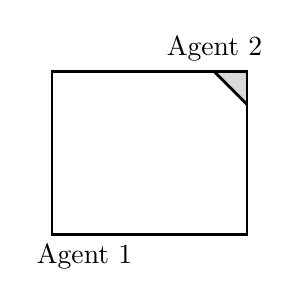
\begin{tikzpicture}[line width=1pt,scale=0.825]
\fill[black!15] (2.5,2.5) -- (3,2.5) -- (3,2);
\draw (2.5,2.5)--(3,2) (0.5,0) node[below]{Agent 1} (2.5,2.5) node[above]{Agent 2};
\draw (0,0) rectangle (3,2.5);
\end{tikzpicture}
\caption{Case with low aggregate risk ($\omega_1=1.2\omega_2$)\label{fig1a}}\vspace{-0.37cm}
\end{subfigure}
\hspace{1.0cm}
\begin{subfigure}[b]{0.6\textwidth}
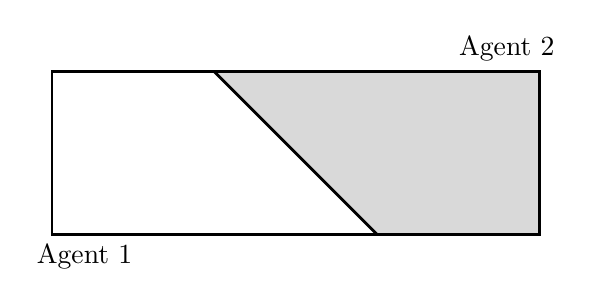
\begin{tikzpicture}[line width=1pt,scale=0.825]
\fill[black!15] (2.5,2.5) -- (5,0)  -- (7.5,0) -- (7.5,2.5);
\draw (2.5,2.5)--(5,0) (0.5,0) node[below]{Agent 1} (7,2.5) node[above]{Agent 2};
\draw (0,0) rectangle (7.5,2.5);
%
\end{tikzpicture}
\caption{Case with large aggregate risk ($\omega_1=3\omega_2$)\label{fig1b}}
\end{subfigure}
%\vspace{-0.5cm}
\end{center}\caption{Endowments distributions where equilibrium exists (gray region) in Example \ref{ex-1} \label{fig1}}
\end{figure}

%\vspace{-0.5cm}
As Figure \ref{fig1} shows, there is a clear difference between economies with substantial risk and economies with almost no risk. For example, in Figure \ref{fig1a}, the Edgeworth Box (EB) has an aggregate risk\footnote{Aggregate risk is defined as the ratio between the aggregate endowments $\omega_1$ and $\omega_2$.} of $20\%$, and as a consequence, the possible endowment distributions in which there is equilibrium are restricted to endowment distributions for agent 2 who is poor compared with agent 1\footnote{Agent 1 might be more than 10 times wealthier than Agent 2.}. This scenario implies that the endowment distributions in which there is an equilibrium compared with all the possible endowment distributions in this EB is quite low, i.e., $1.67\%$. However when there is a large amount of aggregate risk, as in Figure \ref{fig1b}, the existence of equilibrium is less affected by large endowment distributions provided to the risk lover, which implies that the endowment distributions in which there is an equilibrium compared with all the possible endowment distributions in Figure \ref{fig1b} is $50\%$.
\begin{remark}
{Notice that the risk lover does not necessarily have an extremely low importance in the economy to an equilibrium to exist since the allocation in which there is equilibrium does not require extremely low endowment allocation as \cite{Aumann2} suggested. Instead, it is needed large amount of aggregate risk to allow the trade between the agents as it was mentioned above.}
\end{remark}



\begin{figure}[h]
\begin{center}
%\vspace{-0.7cm}
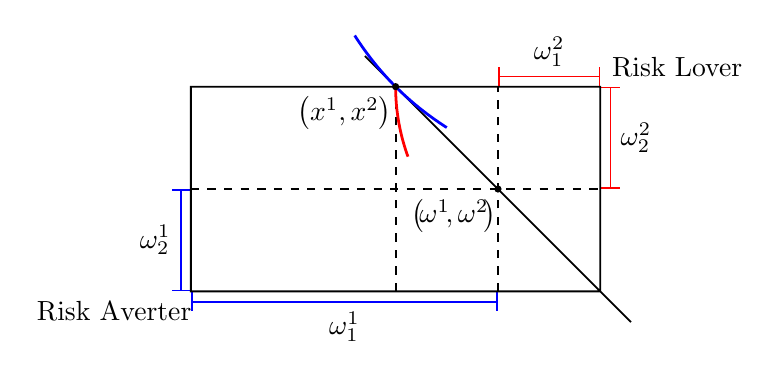
\begin{tikzpicture}[scale=1.3,line width=0.65pt]
\draw[|-|,blue] (0,-0.1) -- (3,-0.1);
\draw[|-|,blue] (-0.1,0) -- (-0.1,1);
\draw[|-|,red] (3,2.1) -- (4,2.1);
\draw[|-|,red] (4.1,1) -- (4.1,2);
\draw (0,0) rectangle (4,2) (1.7,2.3) -- (4.3,-0.3) (1.5,-0.1) node[below]{$\omega_1^1$} (-0.1,0.5) node[left]{$\omega_2^1$} (4.1,1.5) node[right]{$\omega^2_2$} (3.5,2.1) node[above]{$\omega^2_1$} (1.5,2) node[below]{$\left(x^1,x^2\right)$} (-0.75,0) node[below]{Risk Averter} (4.75,2) node[above]{Risk Lover} (2.57,1) node[below]{$\left(\!\omega^1\!,\omega^2\!\right)$};
\draw[dashed] (0,1) -- (4,1) (3,0) -- (3,2) (2,0) -- (2,2);
\draw[domain=1.6:2.5,blue, line width=1pt] plot(\x,4/\x);
\draw[domain=180:200,xshift=4cm,yshift=2cm,red,line width=1pt] plot({2*cos(\x)},{2*sin(\x)});
\fill (2,2) circle (1pt) (3,1) circle (1pt);
\end{tikzpicture}
\end{center}%\vspace{-0.7cm}
\caption{Edgeworth box\label{figEB}}
\end{figure}


This situation suggests as in Figure \ref{figEB} that the existence of equilibrium is strongly related to the aggregate risk that exists in the economy and the wealth that is given to each agent, which increases the possibility of its existence when the endowments are in the hands of the risk averse.




\section{Equilibrium with non-convex agents: General case}
\label{section2}
\subsection{Model}
Let us begin this section by making some comments and notations related to the economies that we will study. Each agent $i$ is characterized by a utility function given by $U^i:\mathbb{R}^S_+\rightarrow\mathbb{R}$ and an Arrow-Debreu constraint given by $px\leq{p}\omega^i$, where $p\in\Delta^{S-1}_+$ is the price and $\omega^i\in \mathbb{R}^S_+$ is the initial endowment for the agent, and each $s=1,\dots,S$ will be interpreted as one state of nature.

We will say that $\left(p,\left(x^i\right)_i\right)$ is an equilibrium (an Arrow-Debreu equilibrium), when $x^i$ is optimal for $U^i$ with the AD-constraint, and also satisfying market clearing, i.e., $\sum_i\omega^i=\sum_ix^i.$



From this point forward, we will consider an economy with $I+J$ agents with two different type of behaviors. The agents $i=1,\dots,I$ are Type $A$ and the agents $j=I+1,\dots,I+J$ are Type $B$.

The agents of Type $A$ have the following:
\begin{A} \label{A1}Utility function, $U^i$, strictly increasing, concave,\end{A}
\begin{A} \label{eqc1} For any $s$ and $\left\{x^n\right\}_{n\in\mathbb{N}}\in\mathbb{R}^S_{+}$, if $x^n_s\rightarrow\infty$ and $\left\{x^n_{s'}\right\}_{n\in\mathbb{N}}$ is bounded for $s'\neq{s}$ then\begin{equation}
\lim_{n\rightarrow\infty}\left(\max_{T\in\partial{U\left(x^n\right)}}\frac{T\circ{e}_s}{T\circ{e}_{s'}}\right)=0\end{equation}where $e_s$ is the canonical vector with 1 in the component $s$ and 0 in any other case.\end{A} \begin{A}\label{eqc2} For any $s,s'$ and $\left\{x^n\right\}_{n\in\mathbb{N}}\in\mathbb{R}^S_{+}$ such that $\left\{x^n_{s}\right\}_{n\in\mathbb{N}},\ \left\{x^n_{s'}\right\}_{n\in\mathbb{N}}$ are bounded from above and bounded away from zero from below then\begin{equation}\liminf_{n\rightarrow\infty}\left(\min_{T\in\partial{U\left(x^n\right)}}\frac{T\circ{e}_{s}}{T\circ{e}_{s'}}\right)\in(0,\infty).\end{equation}
\end{A}

A\ref{eqc1} can be interpreted in terms of the marginal substitution rate between states $s$ and $s'$, i.e., when consumption is moving toward infinity in one state, marginal demand in that state is moving to zero compared to a state with bounded consumption. And A\ref{eqc2} can be interpreted as finite and bounded away from zero marginal demand between states with bounded consumption that is far from zero.


{Intuitively, these two conditions imply that there is some type of independence among the states or goods in the economy because the consumption being arbitrarily large in some of them, does not nullify the marginal utility of consuming any other good or state. And in other words, there are no completely substitutable states or goods in the economy.}

For the agents of Type $B$:
\begin{B} The utility function is strictly increasing and convex.\end{B}


The endowments are given by $\left(\omega_1^i,\dots,\omega_S^i\right)\gg0$. And let us denote $\omega_s:=\sum_{i=1}^{I+J}\omega_s^i,\ \forall{s=1,\dots,S}$.

Because type $B$ agents have convex utility functions, they have the incentive to specialize their consumption as much as possible. However, the agents of type $A$ behave in such a manner so as not to absorb a large amount of risk in their optimal consumption. Because there are two completely opposite attitudes toward risk in which one tends to buy a large amount of risk, it might be desirable for a central planner to reduce the type of specialization that the agents of type $B$ ($I+1\leq{i}\leq{I}+J$) would make. One possible way is to force them to have minimal consumption $\underline{\lambda}_s^i:=\gamma^i\omega^i_s$ for each $s=1,\dots,S$ with $\gamma^i\in\left[0,1\right]$ to avoid extreme consumption in equilibrium. Note that if $\underline{\lambda}^i_s=0\ \forall{i}$, we will have a traditional AD economy without any additional constraint. Therefore we have

\begin{lemma}
Given price $p$, all the $B$ agents have an optimal solution given by:\[x^i_s=\Bigg\{\begin{array}{l} \underline{\lambda}^i_s\ \ \ \ \ \ \ \ \ \ \ \ \ \ \ \ \ \ \ \ \ \ \ \ \ \ \ \ \ \ \textrm{for }{s}\neq s_0\ \textrm{(minimal consumption)}, \\ \frac{1}{p_{s^{\,}_{0_{\,}}}}\left[p\omega^i-\sum_{s\neq{s}_0}p_s\underline{\lambda}^{i^{\,^{\,}}}_s\right]\ \ \ \,\textrm{for some }s_0.\end{array}\]\label{lemmaL}
\end{lemma}
The proof can be found in Appendix \ref{prooflemmaL}.

Another possible requirement is to prohibit agents of type $B$ to take a large amount of risk by imposing a rationing in the consumption ($x^i_s\leq\overline{\lambda}^i_s:=\delta^i\omega_s^i$ where $\delta^i\in[1,\infty]$) that forces the agents to specialize in a larger number of states instead.\footnote{We are grateful to professor Azariadis for this suggestion.}


{One considers this type of constraints as a type of regulation made by a social planner who is worried about the amount of risk that the $B$ agents are consuming. Additionally, if we interpret these agents as gamblers or financial institutions, we may think these constraints as a form to impose capital requirements.}

{One possible reason to impose the constraints mentioned above is that the social planner is worried about the ex post welfare when ``bad'' states occur in which $B$ agents will disappear from the economy.}


{As in Example \ref{ex-1}, we will show that the existence of aggregate risk helps the match of the hedging for type $A$ agents and the speculation of type $B$ agents. However, the former agents must have proportionally more wealth in one state to allow the specialization of the latter without violating market clearing.} Theorem \ref{theo1} ensures this intuition in absence of \emph{rationing} and a nonnegative \emph{minimal consumption}.

\begin{thm}
\label{theo1}
{If the aggregate endowment of type $A$ agents is sufficiently large in a state $s$ compared with other states, there is an equilibrium for the economy.}

\end{thm}

{The proof can be found in Appendix \ref{prooftheo1}. Notice that, in the proof of Theorem \ref{theo1}, the condition described above for the minimal consumption, $\underline{\lambda}^i_s=\gamma^i\omega^i_s$ for $\gamma^i\leq1$, could be relaxed; it is only required that the minimal consumption is lower or equal to the endowment of the agent in each state, $\underline{\lambda}^i_s\leq\omega^i_s$ for all $s$.}

As it was mentioned above, Hypotheses A\ref{eqc1} and A\ref{eqc2} imply some type of independence among states or goods, which would help with the existence of equilibrium when there are type \emph{B} agents.


Our results indicate that when there is enough wealth in one state for the $A$ agents, they are willing to transfer this new risk as much as they can to the $B$ agents, which allows the latter to improve their consumption. Then, even in the presence of non-convex preferences, we will show that there is a balance among the agents given by the presence of this type of aggregate risk.


Notice that this regulation in Theorem \ref{theo1} reduces the level of risk needed in the economy to have an equilibrium since less endowment is needed for \emph{A} agents to ensure market clearing due to the lower available wealth for consuming of the \emph{B} agents.


Given the analysis above, it can be noticed that having high minimal consumption will reduce the level of aggregate risk.

\begin{prop}
\label{prop+mincons}
Under the assumptions of Theorem \ref{theo1}, if there is an endowment distribution in which there is an equilibrium with a minimal consumption given by $\left\{\underline{\lambda}^i_s\right\}_s$, there is an equilibrium for the economy with $\left\{\underline{\lambda}'^i_s\right\}_s$ where $\underline{\lambda}'^i_s\geq\underline{\lambda}^i_s$.
\end{prop}

{However, if the conditions of Theorem \ref{theo1} are not satisfied, this is not true} when there is heterogeneity among the utility functions of the \emph{B} agents and their endowment distributions. This a consequence of the fact that even little perturbations of the minimal consumption constraint could generate a large variation of their consumptions preventing market clearing. {Example \ref{example3agents} in the Appendix, shows that almost any level of minimal consumption will prevent the existence of equilibrium.}


{For economies with both types of regulation, the necessary aggregate risk is possibly in several states depending on each type.} In fact, a strong rationing and a low minimal consumption imply the necessity of aggregate risk in a large amount of states, however, in this case, it is not necessary to have a large level of aggregate risk, that is, the variation among states is not necessarily as large as in Theorem \ref{theo1}. {The intuition behind this is that, in presence of strong rationing and low minimal consumptions, the \emph{B} agents will specialize in a large number of states instead, implying that the level of aggregate risk needed within the states in which they are specializing is lower compared to the case without rationing.}


{As can be seen in Remark \ref{remark1}, rationing of risk does not have properties as the minimal consumption when the regulation is more restricted, see Proposition \ref{prop+mincons}.}

\begin{remark}
\label{remark1}
{A stronger rationing does not ensure an equilibrium since it could require a different endowment distribution to ensure an equilibrium, this is due to the fact that stronger constraints for the \emph{B} agents could increase the number of states in which they are specializing.}
\end{remark}


However, there is relationship between the two types of regulation.
\begin{remark}
{If there is an equilibrium allocation with the minimal consumption $\left\{\underline{\lambda}^i_s\right\}_s$, the same equilibrium allocation can be implemented with rationing instead. And vice versa, if there is an equilibrium allocation with rationing given by $\left\{\overline{\lambda}^i_s\right\}_s$, the same equilibrium allocation can be implemented with minimal consumption instead.}
\end{remark}




Proposition \ref{prop+mincons} suggests that the number of allocations in which we have equilibrium increases when the minimal consumption increases. {However, Proposition \ref{propnoexistence} ensures that, for every level of regulation, equilibrium do not exist for all endowment distributions.}

\begin{prop}
\label{propnoexistence}
For every level of minimal consumption $\left\{\gamma^i\right\}_i$ or level of rationing in the consumption $\left\{\delta^i\right\}_i$, there is an endowment distribution, $\left\{\omega^i\right\}_{i=1}^{I+J}\gg0$, for which there is no equilibrium unless $\gamma^i=1$ or $\delta^i=1$ for all \emph{B} agents.
\end{prop}

Proposition \ref{propnoexistence} says that even in presence of a high level of regulation, it is possible to find endowment allocations for which there is no equilibrium.% However, it does not imply that in some cases, as in Theorem \ref{theo1}, an economy with a certain endowment distribution always has equilibrium with a large regulation.




\subsection{Equilibrium with General Decision Makers}
\label{subsection3}
This section shows that Theorem \ref{theo1} will imply the existence of equilibrium when there are ambiguity lovers and averse agents. We analyze mainly the \emph{SA} Model, \emph{CEU} and \emph{VPs}; in addition, the special case without ambiguity with common priors, which has special features, will also be analyzed.

To have  hypotheses A\ref{eqc1} and A\ref{eqc2} for all the cases below, it seems that it is necessary to assume -- ``roughly'' speaking -- that the marginal utility at a given state $s$ tends towards $0$ when the consumption is moving to infinity in this state.

\subsubsection{SA decision maker}

Every decision maker under SA, see \cite{KMM}, has a probability measure $\mu^i$ over the space of probabilities $\Delta_i\subseteq\Delta_+^{S-1}$, i.e., the space of probabilities that the agent is taking into account, and we can interpret $\mu^i$ as the weight, or importance, that each agent gives to each possible "real probability" or prior that the agent considers plausible.

We will assume that:
\begin{SA}\label{SA1}There exists $\underline{\pi}>0$ such that for each $i$ and $\pi\in\Delta_i$, $\pi_s\geq\underline{\pi}$. \end{SA}Which means that each state has a uniform minimum likelihood that is positive. % and also must be satisfied to avoid arbitrage in the market, which would make the existence of equilibrium impossible.
The previous condition is stronger than $\pi_s>0\ \forall{s}$ since it allows the existence of sequences of probability measures such that $\left\{\pi^n\right\}_{n\in\mathbb{N}}\in\Delta_i$ and $\pi_s^n\rightarrow_n0$. This problem can be eliminated by also assuming that $\Delta_i$ is a closed set.

The agent preference is represented by  $U^i$ which has the form of an SA utility with utility index ${u^i}$ and distortion $\phi_i$ for each $i=1,\dots,I+J$ then
\[
U^i(x)=\int_{\Delta_i}\phi_i\left(\sum_{s=1}^S{u^i}\left(x_s\right)\pi_s\right)\mu^i(d\pi),
\]
where $x\in\mathbb{R}_+^S$, ${u^i}:\mathbb{R}_+\rightarrow\mathbb{R}$, $\phi_i:\mathbb{R}\rightarrow\mathbb{R}$. For $i\leq{I}$ (Ambiguity Averse), \begin{SA}\label{SA2}${u^i}$ and $\phi_i$ are strictly monotone, concave, $C^1$ and ${u^i}$ satisfies $\lim_{x\rightarrow\infty}{u^i}'(x)=0$.\end{SA} For $i$, such that $I<i\leq{I}+J$ (Ambiguity Lovers), \begin{SA}\label{SA3}${u^i}$ and $\phi_i$ are strictly monotone and convex.\end{SA}

\begin{prop}
SA\ref{SA1} and SA\ref{SA2} implies A\ref{A1}, A\ref{eqc1} and A\ref{eqc2}.
\end{prop}
\begin{proof}
Since we have $\pi_s\geq\underline{\pi}>0$ and\[\frac{\partial}{\partial{x_{s'}}}{U^i}(x)=\int_{\Delta_i}\phi_i'\left(\sum_{s=1}^S{u^i}\left(x_s\right)\pi_s\right){u^i}'\left(x_{s'}\right)\pi_s\mu^i(d\pi),\]
then we have A\ref{A1}, and since we have $\frac{\underline{\pi}{u^i}'\!\!\left(x_{s}\right)}{\left(1-\underline{\pi}\right){u^i}'\!\!\left(x_{s'}\right)}\leq\frac{\frac{\partial}{\partial{x_{s}}}{U^i}(x)}{\frac{\partial}{\partial{x_{s'}}}{U^i}(x)}\leq\frac{\left(1-\underline{\pi}\right){u^i}'\!\!\left(x_{s}\right)}{\underline{\pi}{u^i}'\!\!\left(x_{s'}\right)}$ and $\lim_{x\rightarrow\infty}{u^i}'(x)=0$, we have A\ref{eqc1} and A\ref{eqc2}.
\end{proof}



\subsubsection{CEU, rank-dependent expected utility and VP}

For the ambiguity averse and ambiguity lovers in the sense of CEU, see \cite{Schmeidler}, each agent $i$ considers different capacities, $\nu^i:\mathcal{P}\left(\mathcal{S}\right)\rightarrow[0,1]$, where $\mathcal{S}=\{1,\dots,S\}$ such that \begin{ceu}\label{CEU1} for each $A\subsetneq{B}\subseteq\mathcal{S}$, $\nu_{i}(B)-\nu_{i}(A)\geq{\underline{\pi}}>0$.\end{ceu}

The utility function for each agent of this type is given by:
\[
U^i(x)=(C)\int_{\mathcal{S}}{u}^i(x_s)\nu^i(ds)={\int}_{-\infty}^0\left(\nu^i\left[{u}^i\circ{x}{\geq}{t}\right]-1\right)dt+\int_0^{\infty}\nu^i\left[{u}^i\circ{x}{\geq}{t}\right]dt
\]
where $x\in\mathbb{R}_+^S$, ${u^i}:\mathbb{R}_+\rightarrow\mathbb{R}$ and for $i=1,\dots,I$ (ambiguity averse or pessimists), \begin{ceu}\label{CEU2}${u^i}$ is strictly monotone, concave, $C^1$ and ${u^i}$ satisfies $\lim_{x\rightarrow\infty}{u^i}'(x)=0$ and $\nu^i$ is a convex capacity,\end{ceu} For $i$, such that $I<i\leq{I}+J$ (ambiguity lovers or optimists), \begin{ceu}\label{CEU3}${u^i}$ is strictly monotone, convex and ${u^i}(0)=0$ and $\nu^i$ is a concave capacity.\end{ceu}

\begin{prop}
\label{propCEU}
CEU\ref{CEU1} and CEU\ref{CEU2} implies A\ref{A1}, A\ref{eqc1} and A\ref{eqc2}.
\end{prop}
\begin{proof}
Since we have $\nu^i(A)-\nu^i(B)\geq\underline{\pi}>0$ for every $\emptyset\subseteq{B}\subsetneq{A}\subseteq\mathcal{S}$ and $u^i$ is strictly increasing, then  we have A\ref{A1}, and for every $T\in\partial{U}^i(x)$, $\frac{\underline{\pi}{u^i}'\!\!\left(x_{s}\right)}{\left(1-\underline{\pi}\right){u^i}'\!\!\left(x_{s'}\right)}\leq\frac{T\circ{e_s}}{T\circ{e_{s'}}}\leq\frac{\left(1-\underline{\pi}\right){u^i}'\!\!\left(x_{s}\right)}{\underline{\pi}{u^i}'\!\!\left(x_{s'}\right)}$ and as a consequence of $\lim_{x\rightarrow\infty}{u^i}'(x)=0$, we have A\ref{eqc1} and A\ref{eqc2}.
\end{proof}



This result can be adapted to rank-dependent expected utility agents (See \cite{Yaari}) as follows:

A given probability $\pi$ for the world such that $\pi_{s}\geq{\underline{\pi}}\ \forall{s}$, each agent $i$ distorts it with a function $f^i$; for the pessimist agent, $f^i$ will be a convex function, and for the optimist, $f^i$ will be a concave function. In addition, $f^i(0)=0$ and $f^i(1)=1$.

The utility function for each agent of this type is given by $U^i(x)=(C)\int{u}^i(x)df^i\circ\pi$, where for $i=I+1,\dots,I$, ${u^i}$ is strictly monotone, concave, $C^1$ and ${u^i}$ satisfies $\lim_{x\rightarrow\infty}{u^i}'(x)=0$, and for $i$, such that $I+J<i\leq{I}+J$, ${u^i}$ is strictly monotone, convex and ${u^i}(0)=0$.

\begin{remark}
If we impose similar conditions as in the SA case for the set of priors and for the utility index, as $\lim_{x\rightarrow\infty}{u^i}'(x)=0$, the previous result can be extended to the ambiguity averse given by VPs, $U^i(x):=\min_{\pi\in\Delta^i}\left(\sum_{s}u\left(x_s\right)\pi_s+c(\pi)\right)$, see \cite{MMR}.
In fact, A\ref{eqc1} and A\ref{eqc2} will be satisfied because for each $\pi\in\Delta^i$, we will have a limitation in a similar form as before depending only on ${u^i}'$ and $\underline{\pi}$; therefore, we will have an analogous bound as in the previous cases.
\end{remark}





\subsubsection{Risk averse and risk lovers}


Now let us analyze the model in which there is no ambiguity, where $I>0$ and $J\geq0$ represent the number of risk averters and the number of risk lovers, respectively.

Every agent has the same probability $\pi\in\Delta_{++}^{S-1}$, and has expected utility (EU) representation $U^i$ with utility index ${u^i}$; this can be the particular case of both types of decision makers analyzed above (the SA and the CEU). For $i\leq{I}$, ${u^i}$ is strictly monotone, concave and $C^1$, and for $i>I$, ${u^i}$ is strictly monotone, convex and ${u^i}(0)=0$.

The next corollary is a consequence of any of the previous cases and the FOC.

\begin{cor}\label{cor3}
Under the condition of Theorem \ref{theo1}, if each risk averse satisfies $\lim_{x\rightarrow0^+}u'(x)=\infty$, the equilibrium price is given by the solution of
\[
\begin{array}{rcl}
p_s\tilde{x}^i+\sum_{\hat{s}\neq{s}}p_{\hat{s}}{{u^i}'}^{-1}\left(\frac{\pi_s}{\pi_{\hat{s}}}\frac{p_{\hat{s}}}{p_s}{u^i}'\left(\tilde{x}^i\right)\right)\!\! & \!\!=\!\! & \!\!p\omega^i\ \forall s=1,\dots,S,\\
\ \ \ \ \ \ \ \ \ \ \ \ \ \ \,\sum_i{{u^i}'}^{-1}\left(\frac{\pi_s}{\pi_{\hat{s}}}\frac{p_{\hat{s}}}{p_s}{u^i}'\left(\tilde{x}^i\right)\right)\!\! & \!\!=\!\! & \!\!\sum_{i=1}^{I+J}\omega_{\hat{s}}^i-\sum_{j=1}^J\lambda^{I+j}_{\hat{s}}\ \forall\hat{s},{s}=1,\dots,S \\ & & \textnormal{\hspace{4cm} with }\hat{s}\neq{s} \end{array}
\]
for all $i=1,\dots,I$, where $\tilde{x}=\left(\tilde{x}^1,\dots,\tilde{x}^I\right)\gg0$ is the consumption of the risk averse in state $s$.% And for $\left\{\omega^i\right\}_{i=1}^I\gg0$, there is always a solution for this system.
\end{cor}

Notice that for $\left\{\omega^i\right\}_{i=1}^I\gg0$, there is always a solution for this system mentioned in Corollary \ref{cor3}.

The previous result can be extended to include the case in which the risk lovers specialize in different states. However, additional conditions must be needed.%, i.e., conditions over the number of risk lovers, their endowments and the type of minimal consumption.

\begin{prop}
\label{propks}
Given $\left\{\omega_s^i\right\}_{s,i}$ if there are $R$ states, $1\leq{s_1},\dots,s_R\leq{S}$ and $0<k<K$, with $K$ sufficiently large such that:
\begin{enumerate}
\item (Symmetry)\label{cond1} The probability, $\pi_{s_r}$, is the same for all $r$ and $J=R\tilde{J}$ with $\tilde{J}\in\mathbb{N}$ and $\omega^{I+j_1}=\omega^{I+j_2}$ for $j_1=\tilde{j}R+l_1$ and $j_2=\tilde{j}R+l_2$ where $1\leq{l}_1,l_2\leq{R}$ and $0\leq\tilde{j}<R$,
\item (Boundedness) $\sum_{i\leq{I}}\omega_{s_r}^i=\sum_{i\leq{I}}\omega^i_{s_{r'}}\geq{K}$ and $\sum_{i>I}\omega_{s_r}^i\leq{k}$ for all $r,r'=1,\dots,R$, and $\sum_{i}\omega_{s'}^i\leq{k}$ for $s'\neq{s}_r$ for all ${r}=1,\dots,R$,
\item (Minimal consumption)\label{cond5} there exists $\alpha\in[0,1]$ such that $\lambda^i_s=\alpha\omega^i_s$ for each $s$ and $i>I$.
\end{enumerate}
Then, there is an equilibrium for the economy with $p\in\Delta_{++}^{S-1}.$
\end{prop}
\begin{proof}
We define a game where each $\tilde{j}R+1,\dots,\left(\tilde{j}+1\right)R$ will specialize in $s_1,\dots,s_R$ respectively. And using \ref{cond1} and \ref{cond5} we ensure that in each Nash Equilibrium, the prices must satisfy $p_{s_1}=\dots=p_{s_R}$, which concludes the proof.
\end{proof}

Thus, the conditions exposed above require strong symmetric properties. The example \ref{example3agents} in Appendix \ref{examples} explores some difficulties of these types of equilibria.

\begin{remark}
For the case with agents that are risk lovers in some states, $S^i_l$, and risk averters in other states, $S^i_a$, existence of equilibrium can be ensured for preferences such that, for all $s\in\cap_{S^i_l\neq\emptyset}S^i_l$, the utility indexes in this state, $u^i_s(x)$, are linear for $x$ large enough. And similar to Theorem \ref{theo1}, some aggregate risk is necessary to ensure an equilibrium; in this case, the necessity of large endowment could be in more than one state. For example, consider an economy in which there is only two agents where $S^{I+1}_l,S^{I+2}_l\neq\emptyset$, and $S^{I+1}_l\cap{S}^{I+2}_l=\emptyset$, then it will be necessary to have two states with a large endowment in hand of the risk averters\footnote{Notice that this condition can be extended to more than two agents without the large symmetric hypothesis of Proposition \ref{propks}.}.
%\begin{enumerate}
%\item \label{cond1}There is one state in which all agents that has states where they are risk lovers, are risk lover (i. e., $\cap_{S^i_l\neq\emptyset}S^i_l\neq\emptyset$), and exists $s\in\cap_{S^i_l\neq\emptyset}S^i_l$ where the utility indexes in this state, $u^i_s(x)$, are linear for $x$ large enough.
%\item \label{cond2}If two agents are risk lovers in one state, they will be risk lovers in the same states (i. e., if $S^i_l\cap S^j_l\neq\emptyset$ then $S^i_l=S^j_l$), and, for all agents that are risk lovers in the same states, there is at least one state $s$ where the utility indexes in this state, $u^i_s(x)$, are convex and, for $x$ large enough, linear. 
%\end{enumerate}
%Condition \ref{cond1} says that the agents with risk lover behavior, must have a common behavior in the states. This suggests that heterogeneity of the states in which the agents are risk lovers could lead to problems to existence of equilibrium since the agents will specialize in different states depending on $S^i_l$ and the fact of having large aggregate risk is not enough to ensure an equilibrium. And under Condition \ref{cond1}, the result of existence of equilibrium will be as in Theorem \ref{theo1}.

%The previous condition can be extended to more than two agentsas if $S^i_l\cap S^j_l\neq\emptyset$ then $S^i_l=S^j_l$, which implies that all agents with a risk lover behavior in some states does not necessarily agree in the states in which they are risk lovers however, they must agree among all the agents that share their attitude toward risk at least one state. Therefore, you will have collections of agents that share all the states where they are risk lovers. Notice that this collections of agents are $2-2$ disjoint and the set of the states in which each group is risk lover are also $2-2$ disjoint, and therefore, to ensure an equilibrium for the economy, we must have some aggregate risk in the form of Theorem \ref{theo1} in more than one state. %, in fact there must be large aggregate endowment in one state of each of the $2-2$ disjoint set of states in which the agents are risk lovers.
%This result is similar to Proposition \ref{propks} however, we do not need the strong symmetric conditions in terms of endowments, priors and minimal consumptions. 
\end{remark}


\subsubsection{Results in the Edgeworth Box}

The two agents have a EU representation, $U^{i}\left(x\right)=\pi u^{i}\left(x_{1}\right)+\left(1-\pi\right)u^{i}\left(x_{2}\right),\ \forall i=1,2,$
where $\pi\!\in\!\left(0,1\right),u^{1}\in\!{C}^{1}\left(0,\infty\right)\cap{C}[0,\infty)$ is the utility index for the first agent, which is strictly increasing, concave in $[0,\infty)$ and $\lim_{x\rightarrow\infty}{u^1}'(x)=0$, and $u^{2}\in{C}[0,\infty)$ is the utility index for the second agent, which is an increasing and convex function satisfying $u^2(0)=0$.

Thus, Theorem \ref{theo1} can be used in this case, although in the EB, it can be proven that there are also necessary and sufficient conditions for the existence of equilibrium.



\begin{prop}
\label{prop1}
Under our hypotheses, including Inada, there is $\underline{\omega}_1^1\geq0$ and $\underline{\omega}_2^1\geq0$ such that:
\begin{enumerate}
\item There is an AD-equilibrium if and only if (a) $\omega_1^1\geq\underline{\omega}_1^1$ and then $x_2^2=0$, or (b) $\omega_2^1\geq\underline{\omega}_2^1$ and then $x_1^2=0$. 

\item There is a unique normalized price $p=(p_1,1-p_1)\in\Delta_{++}^1$ for the AD-equilibrium, which is the solution of
\begin{equation}
\label{eq:-2}
\omega_1^1={{u^1}'}^{(-1)}\left(\left(\frac{p_1}{1-p_1}\right)\left(\frac{1-\pi}{\pi}\right){u^1}'\left(\omega_2\right)\right)+\frac{1-p_1}{p_1}\omega_2^2
%\omega_1^1={{u^1}'}^{(-1)}\left(\left(\left(\frac{p}{1-p}\right)\left(\frac{1-\pi}{\pi}\right){u^1}'\left(\omega_2\right)\right)\bigwedge{{u^1}'}(0)\right)+\frac{1-p}{p}\omega_2^2
\end{equation}
for (a), and the solution of
\begin{equation}
\label{eq:-21}
\omega_2^1={{u^1}'}^{(-1)}\left(\left(\frac{1-p_1}{p_1}\right)\left(\frac{\pi}{1-\pi}\right){u^1}'\left(\omega_1\right)\right)+\frac{p_1}{1-p_1}\omega_1^2
%\omega_2^1={{u^1}'}^{(-1)}\left(\left(\left(\frac{1-p}{p}\right)\left(\frac{\pi}{1-\pi}\right){u^1}'\left(\omega_1\right)\right)\bigwedge{{u^1}'}(0)\right)+\frac{p}{1-p}\omega_1^2
\end{equation}
for (b).
\end{enumerate}
\end{prop}
The proof of Proposition \ref{prop1} is in Appendix \ref{appA1}.


\begin{remark}
$\underline{\omega}_1^1$ and $\underline{\omega}_2^1$ are the values one would obtain for $\omega_1^1$ and $\omega_2^1$ respectively in \ref{eq:-2} and in \ref{eq:-21} taking $p$ as the solution of $\pi{u}^2\left(\nicefrac{p\omega^2}{p_1}\right)=(1-\pi)u^2\left(\nicefrac{p\omega^2}{(1-p_1)}\right)$.
Thus, $\underline{\omega}^1_1$ depends on all the other endowments of the economy, as for $\underline{\omega}^1_2$.
\end{remark}

\begin{remark}
\label{remarknoInada}The previous result can be extended for a utility index that does not satisfy Inada. Then for condition \ref{eq:-2}, we have 
\begin{equation}
\label{eq:-2n}
\omega_1^1={{u^1}'}^{(-1)}\left(\left(\left(\frac{p_1}{1-p_1}\right)\left(\frac{1-\pi}{\pi}\right){u^1}'\left(\omega_2\right)\right)\bigwedge{{u^1}'}(0)\right)+\frac{1-p_1}{p_1}\omega_2^2
\end{equation}
 and for condition \ref{eq:-21}, we have 
 \begin{equation}
 \label{eq:-21n}
 \omega_2^1={{u^1}'}^{(-1)}\left(\left(\left(\frac{1-p_1}{p_1}\right)\left(\frac{\pi}{1-\pi}\right){u^1}'\left(\omega_1\right)\right)\bigwedge{{u^1}'}(0)\right)+\frac{p_1}{1-p_1}\omega_1^2.
 \end{equation}
\end{remark}



The necessary and sufficient conditions of Proposition \ref{prop1} not only characterize the existence of equilibrium but also ensures its uniqueness. In addition, it helps us to compute the equilibrium price and the optimal consumption for every equilibrium in this economy.

Proposition \ref{prop1} shows that, to ensure the existence of equilibrium, a minimum level of endowment for the risk averse is necessary; then, for every economy with a larger endowment $\omega_1^1$, there is an AD-equilibrium. Therefore, if we have economies in which the aggregate risk is relatively large and most of this wealth is in the hands of the risk averse\footnote{In the sense of possession of large amount of the aggregate risk.}, equilibrium would exist as a consequence of the exchange of risk with the risk lover. Thus, in the presence of risk lovers, it is desirable to have some level of aggregate risk that can be absorbed by the risk lovers without interfering with market clearing. However, in some special cases, an equilibrium can exist in economies with no aggregate risk, see Example \ref{examplenoaggrisk} in Appendix \ref{examples} and Remark \ref{remark8} .



\begin{remark}
\label{remark8}
The conditions exposed in Proposition \ref{prop1} might lead to the existence of equilibrium even when there is no aggregate risk. However, these cases are quite unrealistic and require arbitrarily large differences among agents. Example\ref{examplenoaggrisk} explores this type of equilibrium.
\end{remark}


%\section{Risk sharing with risk lovers and optimists}
%\label{section6}
%As in \cite{Chateauneuf} and in \cite{SW}, to guarantee risk sharing among the risk averters it is necessary that each agent believes in the same probability of the world. To guarantee risk sharing among the ambiguity averters in a model with finite states of natures, each agent believes in the same capacity.
%
%For a continuum of states, Tsanakas et al. proved that using Yaari distortions even with different distortions for the agents, risk sharing occurs when the endowments and the consumption space have non-negative density.% and they also provided a characterization of the equilibrium price and the optimal portfolio in terms of both, aggregate risk aversion and aggregate ambiguity aversion.
%
%For non-convex economies, the analysis of risk sharing is even more difficult. Our goal will be to establish some conditions to ensure that agents are sharing their risk.
%
%
%To analyze the properties of risk sharing, let us define a concept that is deeply related to it: comonotonicity.
%
%
%\begin{definition}
%
%For a consumption plan $x:=\left(x^i\right)_{i=1}^I$, we say that $x$ is \emph{comonotonic} if $x$ satisfies for every $1\leq{i},\ \hat{i}\leq{I}$ and $1\leq{s},\ \hat{s}\leq{S}$, $\left(x^{\hat{i}}_{{s}}-x^{\hat{i}}_{\hat{s}}\right)\left(x^{{i}}_{{s}}-x^{{i}}_{\hat{s}}\right)\geq0$.
%
%\end{definition}
%
%We are interested in the analysis of this property because it is a useful form to compute the optimal consumption, the FOCs and the relationships among prices, aggregate risk and ambiguity found in the economy.
%
%
%
%\subsection{RDEU decision makers}
%
%
%In this case, it is possible to ensure comonotonicity under conditions that can be explained as a generalization of the results mentioned above. In addition, it is possible to characterize the equilibrium price in terms of the endowments, risk aversion and ambiguity aversion that exist in the economy.
%
%\begin{prop}
%\label{prop8}
%If $\left(\omega^i\right)_i$ satisfies the condition of the Proposition \ref{propCEU} on page \pageref{propCEU} with no survival consumption for preferences in the sense of \cite{Yaari}, the consumption is comonotonic if one of the following two conditions is satisfied:
%
%\begin{enumerate}
%\item $\pi_s\geq\pi_{\hat{s}},\ \forall{\hat{s}}\leq{S}$ and there is at least one agent $i\leq{I}$ such that $f^i(x)=x$.
%
%
%\item $\pi_s<\pi_{\hat{s}}$ for some $\hat{s}$, and $K$ (the one that is given in the proof of Theorem \ref{theo1}), is large enough.
%\end{enumerate}
%\end{prop}
%
%
%
%Under the conditions of Theorem \ref{theo1} and Proposition \ref{prop8}, the agents have comonotonic behavior among themselves. However, if the conditions of Proposition \ref{prop8} are not satisfied, agents will have comonotonic behaviors among the agents with similar types of utility function, i.e., among the ambiguity lovers or optimists and among the ambiguity averters or pessimists as it is showed in Example \ref{examplenocomonotonicity} in Appendix \ref{examples}.
%
%Notice that the lack of comonotonicity is a consequence of the low aggregate risk that the economy has compared to the wealth in hands of the risk or ambiguity lovers since their extreme consumption changes the aggregate quantities of goods available for the risk or ambiguity averse to consume.
%
%
%Now, under the conditions mentioned above, we can develop an explicit formula for the utility function that helps us compute the FOC for each pessimist agent. We can then use it to find an expression for the equilibrium price that is an extension of \cite{Buhlmann1,Buhlmann2} and \cite{Tsanakas} to include the case with risk or ambiguity lovers.
%
%
%\begin{prop}
%\label{prop9}
%For $\omega_1>\omega_2>\dots>\omega_S$, CARA RDEU decision makers with $\rho^i>0$ the risk aversion coefficient(for pessimist agents only) with a distortion $f^i$. Under the conditions of the Proposition \ref{prop8} for the state $s=1$ with $x^i\gg0\ \forall{i}\leq{I}$, the equilibrium prices satisfy:
%\begin{equation}\label{eqprice}
%p_s=\frac{e^{-\rho\hat{\omega}_s}e^{\beta_s}}{\sum_{t=1}^Se^{-\rho\hat{\omega}_t}e^{\beta_t}},
%\end{equation}
%where $\frac{1}{\rho}=\sum_{i=1}^I\frac{1}{\rho_i}$, $\beta_s=\rho\sum_{i=1}^I\frac{1}{\rho_i}\ln\left(f^i\left(\sum_{t=1}^{s}\pi_t\right)-f^i\left(\sum_{t=1}^{s-1}\pi_t\right)\right)$, $\hat{\omega}_1:=\omega_1-\sum_{i=I+1}^Jx_1^i=\omega_1-\sum_{i=I+1}^J\frac{(p_1,\dots,p_S)\omega^i}{p_1}$ and $\hat{\omega}_s:=\omega_s$ for $2\leq{s}\leq{S}$.
%\end{prop}
%
%The proofs of Proposition \ref{prop8} and Proposition \ref{prop9} can be found in Appendix \ref{appC}.
%
%\begin{remark}
%We can show that:
%\begin{itemize}\item $\rho$ can be interpreted as the risk aversion coefficient for the ambiguity averse or pessimist; \item $\left\{\beta_s\right\}$ are the coefficients that represent the form in which the ambiguity aversion affects the probability of the world and the equilibrium price; in fact, if $f^i(x)=x\ \forall{i}\leq{I}$, $\beta_s=\ln\pi_s\ \forall{s}$; \item The previous results can be extended to nonnegative minimal consumption such that $\sum_{i=I+j}^{I+J}\lambda^i_1\leq\sum_{i=I+j}^{I+J}\lambda^i_2\leq\dots\leq\sum_{i=I+j}^{I+J}\lambda^i_{S}$, and in this case we have that $\hat{\omega}_s=\omega_s-\sum_{i=I+j}^{I+J}\lambda^i_s$.
%\end{itemize}
%
%\end{remark}
%
%
%Due to the impossibility of deriving a formula that can be easily used to compute the FOC with RDEU agents, we have stated some conditions to ensure comonotonicity among the agents and as a consequence, also with the aggregate endowment distribution. %Therefore, we will assume this type of properties to enable the equilibrium price analysis.
%
%Although the exponential case is idiosyncratic, it helps us show the relationship among aggregate risk, risk aversion coefficient $\rho$, ambiguity in terms of the distortion of each pessimist agent and the equilibrium price.
%
%\section{Volatility and regulation with risk or ambiguity lovers}
%\label{sectionv}
%\label{sectionreg}
%
%
%Now, to analyze changes in volatility through variation of regulation, it is necessary to have financial markets and to establish the type of regulation that we will use. The former will be defined among this subsection. The latter is related to Lemma \ref{lemmaL} in page \pageref{lemmaL} which establishes that every R/A L (risk/ambiguity lover) aims to have an extreme consumption, implying a large specialization for this agent, something that a social planner might find undesirable due to a possible collapse of the economy; and then, one possible form to avoid this type of extreme consumption is by imposing a constraint that prohibits excessive specialization (see Equation \ref{budget1}).
%
%Similarly to section \ref{section2}, let us consider $I+J$ agents where each agent $i$ is a R/A A (risk/ambiguity averse) for $i=1,\dots,I$, and each agent $I+j$ is a R/A L for $j=1,\dots,J$. For simplicity, consider two dates ($t=0$ and $t=1$) and two possible states of nature at the second date. We will suppose that the economy is richer in state 1 (i.e., $\omega_1 > \omega_2)).$ Let $\pi_1 \in (0,1)$ be the objective probability\footnote{If all agents have common beliefs regarding the probability of future events, then the utility function is computed based on common probability $(\pi_1,1-\pi_1)$.} of state 1.
%
%To define the financial structure that we will use, let us interpret the AD equilibria described in Section \ref{section2}, page \pageref{section2}, as the equilibria of an economy with complete financial markets.
%At the first date, there are two real assets: a risk-free asset (which will be called the bond) with a unitary price at $t=0$ and whose payoff at $t=1$ is $R > 0$; and a risky asset with price $q>0$ at $t=0$ and payoff $R_s$ at $t=1$, if state $s$ occurs. Let us assume that $R_1>R_2 \geq 0.$ Thus, the risky asset and the aggregate endowment are comonotonic.
%Each agent $i$ will choose at $t=0$ a portfolio $\varphi=(\alpha,\beta) \in \mathbb{R}^2$, consisting of an amount $\alpha$ of risky asset and an amount $\beta$ of the bond given an initial portfolio $\varphi_0^i=\left(\alpha^i_0,\beta^i_0\right)$ where $\alpha^i_0:=(\omega^i_1-\omega^i_2)/(R_1-R_2)$ and $\beta^i_0:=(\omega^i_2R_1-\omega^i_1R_2)/(R(R_1-R_2))$. The agent's objective is to maximize $V^i(\varphi):=U^i\circ (\varphi A),$ where $A$ is the matrix of payoffs $\left(\begin{array}{cc}
%R_1&R_2\\
%R&R
%\end{array}\right),$
%under the following budget constraints:
%$\varphi$ must be such that 
%\begin{itemize}
%\item[-] Given the risky asset price $q$, \begin{equation}\label{budget0}
%\left(\alpha-\alpha^i_0\right) q + \left(\beta-\beta^i_0\right) =0.
%\end{equation}
%\item[-] For each $s$ at $t=1,$
%\begin{equation}\label{budget1}
%R_s\alpha +R\beta \geq \lambda^i_s,
%\end{equation}
%in other words, at each state $s$, the private wealth after adding the portfolio payoff is exogenously bounded from below by $\lambda^i_s \in [0,\omega^i_s]$ (where $\lambda^i_s=0$ for all $i=1,\dots,I$) this implies that the consumption in each state is bounded from below  for all the R/A L as it was mentioned in section \ref{section2}, and it will be interpreted as a minimal wealth requirement imposed by the policy maker that will be called as \emph{regulation}. And as it was explained above, the reason to impose this type of constraint is that the policy maker or central planner might want to reduce the risk that the risk lovers absorve to avoid possibly the collapse of the economy.
%This situation is related to typical capital requirements for financial institutions.
%As it depends on $s$, it could be picked to be anti-comonotonic with respect to the aggregate wealth as the counter$-$cyclical buffers.% on the Basel III accords (see ...).
%
%%EXPLAIN AGAIN THAT THE REGULATION IS FOR THE RISK LOVER!!!
%
%%EXPLAIN AGAIN THE MODEL
%\end{itemize}
%An equilibrium for this economy will be an asset price $\overline{q}$ and a vector of portfolios $(\varphi^i)_{i=1}^{I+J}$ such that
%\begin{itemize}
%\item[(i)] $\forall i,$ $\varphi^i=(\alpha^i,\beta^i) \in \arg\max \{ V^i(\varphi) : \varphi\in \mathbb{R}^2 $ satisfies $(\ref{budget0})$ and $(\ref{budget1})$ with $ q=\overline{q}\}.$
%\item[(ii)] $\sum_{i=1}^{I+J} \alpha^i=\sum_{i=1}^{I+J} \alpha^i_0$ \, and  \,$\sum_{i=1}^{I+J} \beta^i=\sum_{i=1}^{I+J} \beta^i_0$.
%\end{itemize}
%Given an equilibrium $((\overline{p}_1,1-\overline{p}_1),(x^i)_i)$ for the AD economy $\mathcal{E}_{AD}=(U^i,\omega^i, \lambda^i)_i,$ it is easy to check that, defining 
%\begin{equation}\label{asset_price}
%q(\overline{p}_1)=\frac{\overline{p}_1R_1+(1-\overline{p}_1)R_2}{R}
%\end{equation}
%and $\varphi^i(x^i)=x^iA^{-1}$, the vector $(q(\overline{p}_1),(\varphi^i(x^i))_i)$ is an equilibrium for the economy with financial markets $\mathcal{E}_{FM} = (A,(V^i,\omega^i,\lambda^i)_i).$ Conversely, if $(\overline{q},(\varphi^i)_i)$ is an equilibrium for $\mathcal{E}_{FM},$ let $\gamma_1$ be the risk-neutral probability of state 1 obtained from $\overline{q}$ and $A.$ Then, $((\gamma_1, 1-\gamma_1),x^i(\varphi^i))_i)$ with $x^i(\varphi^i)=\varphi^i A$ is an equilibrium for $\mathcal{E}_{AD}.$ Thus, there is a one-to-one mapping between the equilibria of these two economies such that (i) it keeps the real allocations and (ii) it converts the normalized equilibrium AD prices into risk-neutral probabilities for the respective equilibrium price of the economy with financial markets, and vice-versa.
% 
%Let us define the volatility of returns\footnote{The definition of volatility is in fact the \emph{absolute deviation} of returns.} at price $q$ by  
%\begin{equation}
%\label{eqvol}
%\sigma(q)=\pi_1 \left|\frac{R_1}{q}-\mu(q)\right| + (1-\pi_1) \left|\frac{R_2}{q}-\mu(q)\right|,
%\end{equation}
%where $\mu(q)=\pi_1\frac{R_1}{q}+(1-\pi_1)\frac{R_2}{q}.$
%Furthermore, if the risky asset price is parameterized using Equation \ref{asset_price}, it will be straightforward to verify that the composed function defined by $\sigma ( q(\rho) )$ for $\rho \in (0,1)$ is decreasing. Thus, the volatility of returns decreases with increases in the respective risk-neutral probability of state 1 for a pro$-$cyclical asset. 
%
%
%
%\subsection{Volatility, regulation and changes in utility level}
%
%\label{vol+reg}
%
%As it was explained in Section \ref{sectionv}, $\lambda^i_s\in\left[0,\omega_s^i\right]$ is the type of regulation imposed on the R/A L ($i\geq{I}+1$) by a central planner to avoid the absorption of large quantities of risk that could lead to collapse of the economy due to the non existence of equilibrium. And the idea of this type of regulation is to avoid that the risk lover becomes extremely specialized in equilibrium.
%
%
%
%
%
%Our goal is to establish a relationship between volatility and regulation\footnote{Regulation in the sense of minimal consumption.}, and also analyze, in some special cases, the impact of regulation on the utility levels.% These relationships are illustrated in the following.
%\begin{example}
%\label{exvol1}
%Consider an economy with a two-state nature ($\pi=0.5$), three RDEU agents, two with a CARA utility index and one with a CARL (constant absolute risk lover) utility index given by $\rho^1=1$, $\rho^2=1.5$ and $\rho^3=-1$, exponential distortion $f^i(z):=\frac{1}{{e^{\tau^i}-1}}\left(e^{\tau^iz}-1\right)$ where $\tau^1=1$, $\tau^2=1.25$ and $\tau^3=-1$, endowments given by $\omega^1=(2,1)$, $\omega^2=(2,1)$ and $\omega^3=(1,1)$\footnote{This allocation satisfies the condition of the Theorem \ref{theo1} for any $\lambda^i_s\in[0,\omega_s^i]$.}, and regulation for the third agent given by $\lambda^3\in[0,1]$, which means that if $\lambda^3=0$, there is no regulation and if $\lambda^3=1$, regulation forces consumption without risk, as given by $(1,1)$.
%\begin{center}
%\begin{figure}[ht]
%\includegraphics[scale=0.31]{UtilityC.pdf}
%\includegraphics[scale=0.31]{VolatityC.pdf}
%%\vspace{-0.7cm}
%\caption{Utility levels and Volatility ($\sigma\left(q\left(p_1\right)\right)$) against Regulation ($\lambda^3$)\label{grapWV}}
%%\vspace{-0.7cm}
%\end{figure}
%\end{center}
%
%
%
%From the analysis of Figure \ref{grapWV}, regulatory changes produce variations in utility levels. However this variation behaves quite differently than regulation in traditional convex economies because all agents lose part of their utility when there is more regulation.
%
%The largest reduction on the utility level is for risk lovers because regulation reduces the quantity of risk that they can absorb in equilibrium, obliging the agent to consume an allocation far from their optimal levels in an unregulated economy. In addition, there is a reduction in the utility level for the ambiguity averters due to a larger amount of the aggregate risk that must be absorbed by ambiguity averters when there is regulation for the ambiguity lovers. This scenario leads to riskier optimal allocations for the ambiguity averse, which will reduce their utility levels.
%
%As a consequence, for any social welfare function that we use, increases in regulation will reduce the social welfare of the economy, suggesting that a regulation that tends to reduce the risk that ambiguity lovers absorb is not a good tool for increasing welfare. However, it could be useful to ensure equilibrium in cases in which there is no a large amount of risk in hand on the R/A averters.
%
%As can be shown empirically, increases in regulation lead to rises in volatility in the presence of R/A L, which is a consequence of the lower level of risk that the risk lovers can absorb when there is regulation.
%
%As indicated above, in presence of ambiguity lovers, aggregate risk is required to allow the trade-off among agents. With assets that are comonotonic with the aggregate endowment, the existence of this risk implies that increases in regulation will decrease the price of the risky asset (see equation \ref{asset_price}) and will increase the volatility as a consequence (see equation \ref{eqvol}).
%
%\end{example}
%
%
%The analysis made above can be generalized, using Proposition \ref{prop9} on page \pageref{prop9}, to more that two states.
%
%
%\begin{prop}
%\label{propv}
%Under the conditions of the Proposition \ref{prop9} and $\sum_{j=1}^J\omega_{s}^{I+j}=\sum_{j=1}^J\omega_{s'}^{I+j}$ for all $1\leq{s},s'\leq{S}$, $p_1$ decreases when the regulation increases as $\lambda^i_s=\alpha\omega^i_s$ for $\alpha\in[0,1]$.
%\end{prop}
%
%The proof of Proposition \ref{propv} is in Appendix \ref{appC}.
%
%Additional assumptions are required that guarantee no aggregate risk for risk lovers or optimists. We conjecture that this assumption can be relaxed to allow some type of aggregate risk for them.
%
%Notice that, under the condition of the Proposition \ref{prop9}, decreases in $p_1$ will imply decreases on volatility due to the large aggregate and the relationship between the prices and volatility, see equation \ref{eqvol}.
%
%Therefore, since risk lovers or optimists have substantial incentives to absorb extant risk in the economy, they will increase the price of the assets that allow them to do so (pro$-$cyclical assets), which tends to reduce volatility in the economy. However, if the regulation does not permit these actions, the price of these assets will decrease because they are considerably less important to the ambiguity averse, leading to increases on volatility under equation \ref{eqvol}.% Thus, regulation will increase volatility because there is more risk that must be absorbed by the risk averters or pessimists.
%
%
%As we indicated above, the previous analysis was made with pro$-$cyclical assets. For counter$-$cyclical assets, larger differences among the state prices will imply less volatility for the risky assets, implying results on the opposite direction.
%
%\textbf{If we apply the analysis mentioned above for these assets, we will have that a social planner worried about the volatility caused by counter$-$cyclical assets could increase regulation on them to do so. Since this is case of most of the assets that can be shorted, the social planner could increase regulation over these assets which could increase the possibility of a crisis in the economy, see (?).}
%
%% This is case of most of the assets that can be shorted.
%
%%\textbf{EXPAND!!!!}
%
%%However, these types of assets are not as common as their counterparts.% because much of the private stock is pro$-$cyclical.
%



%
%\subsection{Changes in Prices and Utility with changes in risk attitude}
%
%{Let us analyze the risk aversion utility level and absolute variation of prices\footnote{By absolute variation of prices, we mean $\left|p_1-1/2\right|+\left|p_2-1/2\right|$.}\footnote{It will also called volatility since this value is comonotonic with the volatility of pro-cyclical assets in a two-datese economy.} when one agent changes its attitude toward risk in an economy with large aggregate risk}. We will change the behavior of one them allowing him to be Risk/Ambiguity Lover (R/A L) or Risk/Ambiguity Averse (R/A A), it means that this agent will vary from risk/ambiguity propension to aversion.
%
%\begin{example}
%\label{exvol2}
%Consider an economy with a two-state nature ($\pi=0.5$), two RDEU agents one with a CARA utility index given by $\rho_1=1$ and another one with a CARA or CARL utility index given by $\rho_2\in[-1,1]$, exponential distortion $f^i(z):=\frac{1}{{e^{\tau^i}-1}}\left(e^{\tau^iz}-1\right)$ where $\tau^1=1$ and $\tau^2=\rho^2$, endowments given by $\omega^1=(4,1)$ and $\omega^2=(2,1)$, and with $\lambda=0$.
%\begin{figure}[ht]
%\begin{center}
%\includegraphics[width=0.49\linewidth]{VolatilityPAa1.pdf}
%\includegraphics[width=0.485\linewidth]{UtilityPAa1.pdf}
%%\vspace{-0.5cm}
%\caption{Utility levels and Absolute variation of prices ($\sigma\left(q\left(p_1\right)\right)$) against R/A coefficient of Agent $2$ ($\rho^2$)\label{grapWV2}}
%%\vspace{-0.7cm}
%\end{center}
%\end{figure}
%%\vspace{-0.4cm}
%
%Figure \ref{grapWV2} shows that changes in $\rho^2$ produce variations in utility levels depending on the risk attitude of agent $2$; when Agent $2$ is R/A Lover, there is no changes in the utility level of Agent $1$ because consumption is the same for all the cases. However, Agent $2$ has large utility losses as he becomes less R/A L when $\rho^2$ is increasing since this agent is reducing his desire for consumption with substantial amounts of risk. However, when the agent become R/A Averse, Agent $2$ is incentivized to consume less risk than before, and due to the amount of risk in the economy, both agents have utility losses. Therefore, in economies with large aggregate risk, it is desirable for the Risk Averters to have some Risk Lovers to absorb most of the risk of the economy.
%
%As we discussed above, there are no changes in equilibrium allocations when Agent $2$ is R/A L because this agent tends to specialize as much as possible, which implies that the optimal allocation does not change. When Agent $2$ becomes R/A A, he is incentivized to avoid too much specialization. However, because the Inada condition is not satisfied, small amount of risk could imply specialization for slightly pessimistic agents. Intuitively, for a R/A A agent with a small $\rho^2$, the incentives to have consumption with low specialization are quite small, and at low levels of risk, the agent would specialize as a risk lover. However when $\rho^2$ is large, the incentives are considerably larger, and extreme specialization is avoided.
%
%Therefore absolute variation is constant for $\rho^2\in[-1,\gamma]$, where $\gamma\approx0.15$ and for $\rho^2>\gamma$, Agent $2$ specializes gradually, forcing Agent $1$ to consume more risk. Since both agents are R/A A
%, they must absorb all the risk, which implies larger differences among state prices as the economy becomes more R/A A, leading to increments of the absolute variation of prices as a consequence.
%\end{example}
%



\section{Equilibrium with Friedman-Savage Decision Makers and other preferences}
\label{sectionfs}
\subsection{Conditions for existence of equilibrium}

In this section we have two types of agents and a finite number of them, $I+J$; nevertheless, we consider Friedman-Savage Decision makers instead of agents with convex utility functions (agents of type B). Thus, we analyze the existence of equilibrium when there are also agents of type A.


{Each Friedman-Savage (FS) Decision Maker $i=I+1,\dots,I+J$ has a subjective probability $\pi^i\in\Delta^{S-1}_{++}$ and a utility index ${u^i_s}:\mathbb{R}_+\rightarrow\mathbb{R}$ for each $s$ that is differentiable, and strictly increasing. Moreover, there are $0\leq{x}^i_{c,s}\leq\tilde{x}^i_s$ such that for each $x<{x^i_{c,s}}$ or $x\geq\tilde{x}^i_s$, ${u^i_s}$ is a concave differentiable function, and, for $x\in\left[x^i_{c,s},\tilde{x}^i_s\right]$, ${u^i_s}$ is a convex function. Then, the utility function has the following form $U^i(x):=\sum_{s=1}^S\pi_s^i{u^i_s}\left(x_s\right)$. The endowments are given by $\left(\omega^i_1,\dots,\omega^i_S\right)\gg0$.}

{This type of agent has a very particular behavior due to the two inflection points, before the first inflection point wherein each FS Decision Maker behaves as risk averse, avoiding extreme consumptions; although, when this agent is wealthier, he will behave as a certain type of risk lover, avoiding consumption without risk, however, if the agent becomes even more wealthier, his attitude toward risk changes again becoming  a risk averter. Intuitively, this implies that he is worried about the extremely low consumptions  even having incentives to specialize at some levels of wealth, and, at the same time, he does not have strong incentives to have a large specialization when their wealth is considerably large; this behavior is supported by several empirical works in which bettors changes their attitude toward risk becoming risk averters for gains  and risk lovers for losses based on a reference point, their wealth as in \cite{JS}.}

%{The agents described above are willing to specify in some states but are also concerned about low consumption in all the states; at the same time, this agents that are willing to absorb risk at some middle level of income but they are not willing to do so when they are in high level of it. }

{This behavior cannot be explained with the previous type of preferences because each B agent is willing to specialize in one state in absence of any type of constraint and its attitude does not depend on the level of wealth.}



\begin{prop}
\label{exisFS}
{If the aggregate endowment of type $A$ agents is sufficiently large in $0<S_1<S$ states compared with other states, there is an equilibrium for the economy.}
%Given a state $1\leq{s}\leq{S}$, there is $K>0$ such that $\sum_{i\leq{I}}\omega_s^i\geq{K}$, and then there is an equilibrium for the economy and the equilibrium price satisfies that $p\in\Delta_{++}^{S-1}.$
\end{prop}

The proof of Proposition \ref{exisFS} is in Appendix \ref{appC}.

\begin{remark}
{For each Friedman-Savage decision maker, if Inada condition holds,
%$\lim_{x\searrow0}{u^i}'(x)=\infty$
 in equilibrium, each DM would have a positive consumption in each state. However, if Inada condition is not satisfied, they might have null consumption in some states even when they have incentives to avoid them.}
\end{remark}

\begin{remark}
{If the endowment for all FSDM is quite small, or quite large, compared to $x^i_c$ and $\tilde{x}^i$ respectively, there is no need to impose a large aggregate endowment difference among states since all of them will consume in the first concave part, or in the second convex part, of the utility function in absence of large aggregate endowments variations among states. In fact, the existence of relatively large variations in this case, could prevent the existence of equilibrium since they could have incentives to consume in the middle region and, if the variation is not large enough, market clearing could be violated.}
\end{remark}

Consider an example that illustrates the fact that the lack of aggregate risk will prevent the existence of equilibrium if the Friedman-Savage agents are not extremely ``poor'' or extremely ``rich''.

\begin{example}
Consider three agents with EU preferences with an objective probability given by $(\pi_1,\pi_2)=(1/2,1/2)$ where Agent 1 has a utility function, $u^1$, strictly increasing and strictly concave, Agents 2 and 3 have the same strictly increasing Friedman-Savage utility functions, $u$, satisfying Inada condition. Additionally, consider endowments, $\left(\omega^i_1,\omega^i_2\right)\gg0$, such that $\omega_1=\omega^1_1+\omega^2_1+\omega^3_1=\omega^1_2,\omega^2_2+\omega^3_2=\omega_2$, that is, there is no aggregate risk in the economy, $\omega^2_1+\omega^2_2\neq\omega^3_1+\omega^3_2$ and $\tilde{x}^i\gg\min_s\left\{\omega^i_s\right\}>x^i_c$ for each $i$.

Let us prove that there is no equilibrium for the economy. To do so, we will prove that any price $p=(p_1,p_2)$ does not support an equilibrium. Notice that $p\gg0$ since the preferences are strictly monotone. If $p_1=p_2$, Agents 2 and 3 will specialize in some state of nature, and to have equilibrium, each agent must specialize in a different state, however, since one of the agents is strictly wealthier than the other agent (w.l.o.g. let it be Agent 2 ), we know using the FOC that $\left|x^2_1-x^2_2\right|>\left|x^3_1-x^3_2\right|$, which prevents the existence of equilibrium.

If $p_1<p_2$, it is easy to see that $x^i_1>x^i_2$ for each agent $i$, which leads to incompatibility with market clearing in an economy without aggregate risk.

\end{example}


%\begin{remark}
%\label{remarkfsext}
%With respect to the general utility index of Friedman and Savage, it is possible to show the existence of equilibrium for agents that are quite poor or considerably rich such that their consumption is always in the concave part of the utility index. \textbf{However, it is possible to extend the Lemma \ref{lemma3} in page \pageref{lemma3} to  all types of FS utility indexes implying that the consumption in the convex part is at most in one state. For agents with consumption in the convex part, the proof of Proposition \ref{exisFS} can not be extended however, numerically can be observed that the result remains true.}
%\end{remark}

\subsection{Static Equilibrium with Prospect Theory}

{Now, let us define a static economy with agents consistent with Prospect Theory as given by \cite{KT92}. Consider an AD economy similar to the one defined before where there is an objective probability $\pi_s>0$ for each state to occur\footnote{Notice that, in our economy, agents can not buy lotteries as in an Ascombe-Aumann framework.}. Since this type of agents considers differently gains and losses based on their personal reference point it is possible to make the analysis for gains and losses separately (gains for levels of wealth above the point and losses for levels of wealth below it).}

{Therefore, if we interpret our economy as a two-dates economy in which, in $t=0$, contracts are made, and, in $t=1$, agents honor their promises; it is natural to think that the reference point is the level of wealth that each agent will have before the contracts are honored in $t=1$, that is $\omega^i_s$, the initial endowment in each state.}
{If the agent does not have any shock in his/her wealth, in any of the possible states, the level of wealth will be constant among the states, $\omega^i_{s}=\omega^i_t$ for all $s,t$, however, if the agent has a shock caused by an external force, the reference points could not be necessarily the same in all states implying a different utility index among the states as a consequence.}

Since these agents change their attitude toward the reference point as we mentioned before, the Friedman-Savage utility index is useful in the analysis of the value function mentioned in the Prospect Theory literature. For the case of \cite{KT92}, we have:

\begin{TK}$U^i$ are given as in Proposition \ref{exisFS} with $x^i_{c,s}\leq0$ and $\tilde{x}^i_s=\omega^{I+j}_s\ \forall{s}$ where $x^i_{c,s}$ and $\tilde{x}^i_s$ are the inflection points for the state $s$.
\end{TK}
However, in this framework, agents can not have arbitrarily large losses since their consumption must be nonnegative in each state as in the classical model. One possible explanation to this is that in a more complex framework than the one considered by the classical Prospect Theory, agents can not have large losses in an environment without default since they are exogenously forced to avoid negative consumption.



{Since the Friedman-Savage preferences have two inflection points that separate the convex part from the concave parts of the utility index, Proposition \ref{exisFS} can be used to analyze economies with agents consistent with the prospect theory in the sense of \cite{KT92} for linear distortions and $x^i_c=0$ since $\tilde{x}^i=\omega^{I+j}_s\ \forall{s}$ could be the reference point mentioned in \cite{KT}. However, it could also include cases in which the agents would like to avoid risk seeking under extremely low levels of wealth as in \cite{JS}:
\begin{JS}
$U^i$ are given as in Proposition \ref{exisFS} with $x^i_{c,s}=\omega^{I+j}_s$ and $\tilde{x}^i_s>\omega^{I+j}_s\ \forall{s}$ where $x^i_{c,s}$ and $\tilde{x}^i_s$ are the inflection points for the state $s$.
\end{JS}


The following result ensures the existence of equilibrium for the preferences described above.


\begin{cor}
\label{corollary}
{For preferences described above under the conditions of Proposition \ref{exisFS}, there is an equilibrium for the economy.}
\end{cor}


\begin{remark}
{To analyze a more general case than the one mentioned above, for example, with nonlinear distortions, the result will be still valid under some additional conditions, for example, conditions that ensure a non constant consumption among the agents and, as a consequence, the utility function can be written in functional form in a neighborhood of the optimal solution. Under these conditions, it can be extended for cases where there are two different distortions which are concave for small probabilities and convex for large probabilities as in \cite{KT92}, \cite{ABW}, \cite{Wakker} or else \cite{JS}.}
\end{remark}

\begin{remark}{For preferences given by Prospect Theory in an economy with infinitely many states, the conditions mentioned above are not sufficient to ensure equilibrium since the distortions for low-probability events could cause some type of arbitrage for standard EU agents or risk-neutral firms with complete markets. In fact, \cite{AG} found conditions to overcome this problem that depend on the asymptotic behavior of the value function and the weighting function, conditions which seems to be empirically unrealistic. These conditions, even being unrealistic, are necessary to ensure optimality of the consumers and firms, therefore, to ensure equilibrium in this framework, the two type of conditions\footnote{Conditions mentioned in \cite{AG} and in Corollary \ref{corollary}.} must be satisfied to ensure market clearing and optimality of all agents, and hence, equilibrium in an economy with a finite number of agents.

However, the conditions explored in their paper seem to be too dependent on the completeness of the markets and the existence of a infinitely number of states, then, since the empirical evidence seems to be non-compatible with these conditions, a model with incomplete markets in an infinite-state model could be the only case compatible with equilibrium with preferences given by Prospect Theory\footnote{Note that a model with an infinite number of states with incomplete markets could lead to an economy with several AD constraints as the one analyzed in our paper.}.}
\end{remark}





\subsection{A numerical analysis of prices with Friedman-Savage preferences}
Because increments on the Friedman-Savage Wealth produce changes in their decisions against risk, our goal will be to establish a relationship between the risk absorbed by them and their wealth and -- as a consequence -- a relationship between prices and wealth of the FS decision makers.% The following example illustrates these relationships.

\begin{example}
Consider an economy with two states of nature with the probability $\pi=0.5$ that the first state occurs, two EU agents, where $u^1(x)=\ln(x)$ and $u^2(x)=\left\{\begin{array}{ll}\ln(x)+(1/2)x^2 & \textnormal{if }x\leq3/2 \\ 13/6(x-3/2)+9/8+\log(3/2) & \textnormal{if }x>3/2,\end{array}\right.$ and endowments given by $\omega^1=(5-2.5a,2-a)$ and $\omega^2=(2.5a,a)$ where $a\in[0,1]$.
\begin{center}
\begin{figure}[ht]
\includegraphics[width=0.48\linewidth]{propconsfs1.pdf}
\includegraphics[width=0.5\linewidth]{volatilityfs1.pdf}
\vspace{-0.3cm}
\caption{Changes in consumption and Absolute Variation of Prices against Wealth\label{grapfs}}
\end{figure}
\end{center}
\vspace{-0.5cm}
From the analysis of the Figure \ref{grapfs}, incremental increases of wealth of the FS agent lead to reductions of the absolute variation of prices. This is a consequence of the increasing desire of this decision maker to specialize when there are incremental increases of his wealth. Under a low wealth condition, the economy will be convex because both agents would have convex preferences under the feasible space. However under a substantial wealth condition, the FS decision maker will have enough incentives to specialize the consumption in one state.

Because we are using allocations in the sense of Proposition \ref{exisFS}, there is some type of aggregate risk in the economy. Therefore, as the Friedman-Savage decision maker is becoming richer, she will have incentives to specialize her consumption and absorb larger quantities of risk, which reduces the volatility of the economy with a pro$-$cyclical asset.



\end{example}




\section{Conclusions}

Given the importance of risk loving in financial markets, the exchange of aggregate risk between risk lovers and the risk averters is an important problem to be studied since it is not typically analyzed in the General Equilibrium Theory. To do so, we gave conditions in terms of enough aggregate risk for a large class of models encompassing \emph{SA} (see \cite{KMM}), \emph{CEU} (see \cite{Schmeidler}), \emph{VPs} (see \cite{MMR}), \cite{FS} -- a type of decision maker that changes its attitude toward risk and that is a risk lover for middle wealth and risk averse for low wealth and substantial wealth conditions -- and some special cases of Prospect Theory\footnote{In the sense of \cite{JS} and \cite{KT92}.} under which we were able to prove the existence of equilibria\footnote{For existence of Pareto Optima see \cite{ABCN}.}. We can interpret this condition as the following: a level of aggregate risk is required to enable trade between risk lovers and risk averters and helps with the matching between the desire of hedging by risk averters and of speculation by risk lovers.

The analysis mentioned above can be useful to analyze theoretically and numerically the influence of Risk Loving or Friedman-Savage preferences in economies with financial markets and how volatility and welfare can be affected by regulation and the amount of risk that exists in the economy.

%We also provided some robust examples that suggest that regulation increases volatility for pro$-$cyclical assets, whereas it reduces the utility levels in economies with large aggregate risk. However, the risk lovers or optimists are those who incur the larger losses. These results are analogous if we have Friedman-Savage agents instead of risk lovers.


 
%We established conditions for risk sharing among agents with RDEU agents with convex distortions $f^i$. They suggest that ambiguity lovers cannot absorb all the risk of the ambiguity averse with enough aggregate risk, which forces the ambiguity averse to consume part of it and allows the risk to be shared among agents.

%Finally, we generalized the results given by \cite{Buhlmann1,Buhlmann2} and \cite{Tsanakas} to the case with ambiguity lovers, and found a characterization of the equilibrium price in terms of the aggregate risk aversion and the ambiguity aversion that exists in the economy.


%All the analyses that were made throughout the paper were in economies with complete markets and without any friction. However, in the presence of frictions, such as incomplete markets and collateral, the result is simply not necessarily true because the risk lovers cannot do all the trades to specialize their consumption as much as possible having a situation similar to the case of rationing, which implies that collateral is not necessarily helpful for the existence of equilibrium with Risk Lovers.% and differs from \cite{DGZ}.
%falar do fato de tirar a referencia

\emph{Araujo: IMPA, Estrada Dona Castorina 110, Jardim Bot\^{a}nico, Rio de Janeiro, RJ 22460-320, Brazil and EPGE/FGV, Praia de Botafogo 190, Botafogo, Rio de Janeiro, RJ 22250-040, Brazil, aloisio@impa.br. Chateauneuf: IPAG Business School and Paris School of Economics, Universit\'{e} de Paris I, 106-112 Boulevard de l'H\^{o}pital, 75647 Paris, France, Alain.Chateauneuf@univ-paris1.fr. Gama-Torres: IMPA, Estrada Dona Castorina 110, Jardim Bot\^{a}nico, Rio de Janeiro, RJ 22460-320, Brazil, jpgamat@impa.br. Novinski: Faculdades Ibmec-RJ, Rio de Janeiro, Brazil, Avenida Presidente Wilson 118, Centro, Rio de Janeiro, RJ 20030-020, Brazil, rodrigo.novinski@ibmecrj.br.}

\appendix

\section{Appendix}
%\subsection{Proofs of existence of equilibrium}
%\label{appA}
\subsection{Proofs of Section \ref{section2}}\label{appA1}

\label{prooflemmaL}
\begin{proof}[Proof of Lemma \ref{lemmaL}]
Since all $B$ agents have a convex utility function, for any $\alpha\in[0,1]$ $U^i(\alpha{x}_1+(1-\alpha)x_2)\leq\alpha{U}^i(x_1)+(1-\alpha)U^i(x_2)\leq\max_t\{U^i(x_t)\}$, which implies that there is an optimal consumption on the boundary of the budget set, and due to the minimal consumption, the budget set is generated by $\left\{\left(\lambda_1,\dots,\frac{1}{p_s}\left[p\omega^i-\sum_{t\neq{s}}p_t\lambda_t,\dots,\lambda_S\right]\right)\right\}_{s=1}^S$.
\end{proof}


\begin{proof}[Proof of Proposition \ref{prop1}]
%Let us assume first Inada for the risk averse.
For any $p_1\in(0,1)$, since the agent 2 has a strictly convex and strictly increasing utility index, the optimal solution must be on the frontier of the budget set therefore the possible optimal solution are $\left(\frac{p\omega^{2}}{p_1},0\right)$ and $\left(0,\frac{p\omega^{2}}{1-p_1}\right)$, see lemma \ref{lemmaL}.

From now on we will analyze the case in which the agent 2 specializes in the first state. Consider $\overline{p}_1\in\left(0,1\right)$ and $\overline{p}=(\overline{p}_1,1-\overline{p}_1)$\footnote{The uniqueness of $\overline{p}_1$ is a consequence of $u^2$ being strictly increasing, $u^2(0)=0$, $u^2(x)\rightarrow\infty$ when $x\rightarrow\infty$, and that the left part of \ref{eq:-3} is decreasing and the right part is increasing with $\overline{p}_1$.} such that 
\begin{equation}
\pi u{}^{2}\left(\frac{\overline{p}\omega^{2}}{\overline{p}_1}\right)=\left(1-\pi\right)u^{2}\left(\frac{\overline{p}\omega^{2}}{1-\overline{p}_1}\right)\label{eq:-3}
\end{equation}
and $\underline{\omega}_{1}^{1}>0$ given by \ref{eq:-2} where $p_1=\overline{p}_1$. Since $\omega(p)={{u^1}'}^{\left(-1\right)}\!\!\left(\!\left(\frac{p}{1-p}\right)\!\!\left(\frac{1-\pi}{\pi}\right)\!{u^1}'\left(\omega_2\right)\right)+\frac{1-p}{p}\omega_2^2$ is strictly decreasing for $p\in(0,1)$, the equation \ref{eq:-2} has a unique solution $p_1$ for each $\omega_1^1$.

Now let us prove that for each $\omega_{1}^{1}\geq\underline{\omega}_{1}^{1}$ there is an equilibrium when the price $(p_1,1-p_1)$ is the solution
of \ref{eq:-2}.

If $\omega_{1}^{1}\geq\underline{\omega}_{1}^{1}$, then $p_1\leq\overline{p}_1$
so $\pi u{}^{2}\left(\frac{p\omega^{2}}{p_1}\right)\geq\left(1-\pi\right)u^{2}\left(\frac{p\omega^{2}}{1-p_1}\right).$

This implies that the optimal consumption of the agent 2 is $\left(\!\frac{p\omega^{2}}{p_1},\!0\!\right)$ given $p$.

Now, the FOC for the first agent implies
$\pi {u^1}'\left(x_{1}^{1}\right)=p_1\mu,$
$\left(1-\pi\right){u^1}'\left(x_{2}^{1}\right)=\left(1-p_1\right)\mu$
and
\begin{equation}
\ \ \ \ \ \ \ \ p_1x_{1}^{1}+\left(1-p_1\right)x_{2}^{1}=p_1\omega_{1}^{1}+\left(1-p_1\right)\omega_{2}^{1},\label{eq:-4}
\end{equation}


for $\mu>0$. If we define $\left(x^1_1,x^1_2\right)=\left({{u^1}'}^{\left(-1\right)}\left(\left(\frac{p}{1-p}\right)\left(\frac{1-\pi}{\pi}\right){u^1}'\left(\omega_2\right)\right),\omega_2\right)$, it is not hard to see that for $\mu=\frac{1-\pi}{1-p}{u^1}'(\omega_2)$, $\left(x^1_1,x^1_2\right)$ is a solution for the FOC mentioned above.
%Therefore, we have 
%\[
%x_{1}^{1}={{u^1}'}^{\left(-1\right)}\left(\left(\frac{p}{1-p}\right)\left(\frac{1-\pi}{\pi}\right){u^1}'\left(x_{2}^{1}\right)\right)
%\]
% and using \ref{eq:-4} we have 
%\begin{equation}
%p{{u^1}'}^{\left(-1\right)}\left(\left(\frac{p}{1-p}\right)\left(\frac{1-\pi}{\pi}\right){u^1}'\left(x_{2}^{1}\right)\right)+\left(1-p\right)x_{2}^{1}=p\omega_{1}^{1}+\left(1-p\right)\omega_{2}^{1},\label{eq:-5}
%\end{equation}
%and using \ref{eq:-2} we have
%\begin{equation}
%p{{u^1}'}^{\left(-1\right)}\left(\left(\frac{p}{1-p}\right)\left(\frac{1-\pi}{\pi}\right){u^1}'\left(x_{2}^{1}\right)\right)+\left(1-p\right)x_{2}^{1}=p{{u^1}'}^{\left(-1\right)}\left(\left(\frac{p}{1-p}\right)\left(\frac{1-\pi}{\pi}\right){u^1}'\left(\omega_{2}\right)\right)+\left(1-p\right)\left(\omega_{2}^{1}+\omega_{2}^{2}\right).
%\label{eq:-6}
%\end{equation}
%
%
%Using the fact that if 
%\[
%f_{p}\left(\omega\right):=p{{u^1}'}^{\left(-1\right)}\left(\left(\frac{p}{1-p}\right)\left(\frac{1-\pi}{\pi}\right){u^1}'\left(\omega\right)\right)+\left(1-p\right)\omega,
%\]
% its derivative is defined by 
%\[
%f'_{p}\left(\omega\right)=\frac{p}{{u^1}''\left({{u^1}'}^{\left(-1\right)}\left(\left(\frac{p}{1-p}\right)\left(\frac{1-\pi}{\pi}\right){u^1}'\left(\omega\right)\right)\right)}\left(\frac{p}{1-p}\right)\left(\frac{1-\pi}{\pi}\right){u^1}''\left(\omega\right)+1-p>0.
%\]
%It implies that $x_{2}^{1}=\omega_{2}$, and that $x_{1}^{1}={{u^1}'}^{\left(-1\right)}\left(\left(\frac{p}{1-p}\right)\left(\frac{1-\pi}{\pi}\right){u^1}'\left(\omega_{2}\right)\right)$.

And since  we have $x^1_2+x^2_2=\omega_2$ and $x^1_1+x^2_1={{u^1}'}^{\left(-1\right)}\left(\left(\frac{p}{1-p}\right)\left(\frac{1-\pi}{\pi}\right){u^1}'\left(\omega_2\right)\right)+\omega_1^2+\frac{1-p}{p}\omega_2^2=\omega_1^1+\omega^2_1$, this concludes the proof of existence of equilibrium when $x^2_1\neq0$. The proof is analogous when $x^2_2\neq0$.

Let us prove the converse, suppose that there is an equilibrium $\left(\hat{p},\ \hat{x}\right)$ for the economy in which $\hat{x}^2_1\neq0$, then $\hat{x}^1_2=\omega_2$. Since we know that $\hat{p}$ satisfies
\[
\pi{u}^2\left(\frac{\hat{p}\omega^2}{\hat{p}_1}\right)-(1-\pi){u}^2\left(\frac{\hat{p}\omega^2}{1-\hat{p}_1}\right)\geq0,
\]
and using that the function $f$ defined by $f(p):=\pi{u}^2\left(\frac{\left({p},1-{p}\right)\omega^2}{{p}}\right)-(1-\pi){u}^2\left(\frac{\left({p},1-{p}\right)\omega^2}{1-{p}}\right)$ is strictly decreasing and that $\overline{p}_1$ is the greatest $p\in(0,1)$ such that the inequality above is satisfied, we have that $\hat{p}_1\leq\overline{p}_1$. And as a consequence of the FOC of the agent $1$, the equation \ref{eq:-2} is implied for $p_1=\hat{p}_1$, and since $\hat{p}_1\leq\overline{p}_1$, we obtain $\omega_1^1\geq\underline{\omega}_1^1$.
%\[
%\omega_1^1={{u^1}'}^{\left(-1\right)}\left(\left(\frac{\hat{p}}{1-\hat{p}}\right)\left(\frac{1-\pi}{\pi}\right){u^1}'\left(\omega_2\right)\right)+\frac{1-\hat{p}}{\hat{p}}\omega_2^2,
%\]
 Which concludes the proof.
%And finally, using \ref{eq:-4} and the optimal consumption for the
%second agent we have that $\left(\left(p,1-p\right),\left(x_{1}^{i},x_{2}^{i}\right)_{i=1,2}\right)$
%is an equilibrium.
\end{proof}
%Now let us not assume Inada, that is, $\lim_{x\searrow0}{u^1}'\left(x\right)={u^1_+}\!'\left(0\right)<+\infty$. And using an analogous reasoning, we will have:
%\subsection{Proof of Remark \ref{remarknoInada}}
\begin{proof}[Proof of Remark \ref{remarknoInada}]
Due to the FOC, to guarantee that agent $1$ has a positive consumption in each state it is enough to show that \begin{equation}
\left(\frac{1-p_1}{p_1}\right)\left(\frac{\pi}{1-\pi}\right){u^1}'\left(\frac{p_1\omega_{1}^{1}+\left(1-p_1\right)\omega_{2}^{1}}{p_1}\right)<{u^1}'\left(0\right)\label{eq:-7}
\end{equation}for any $p_1\leq\overline{p}_1$ where $\omega_1^1$ satisfies the equation \ref{eq:-2n}. And since ${u^1}'$ is strictly decreasing and $\omega^1_2>0$, we have\[\left(\frac{1-p_1}{p_1}\right)\left(\frac{\pi}{1-\pi}\right){u^1}'\left(\frac{p_1\omega_{1}^{1}+\left(1-p_1\right)\omega_{2}^{1}}{p_1}\right)<\frac{(1-p_1)\pi}{p_1(1-\pi)}{u^1}'\left(\omega^1_1\right)\]
and then, using \ref{eq:-2n}, we have:
\[
\frac{(1-p_1)\pi}{p_1(1-\pi)}{u^1}'\left(\omega^1_1\right)<\frac{(1-p_1)\pi}{p_1(1-\pi)}\left(\left(\frac{p_1(1-\pi)}{(1-p_1)\pi}{u^1}'\left(\omega_{2}\right)\right)\wedge{u^1}'\left(0\right)\right)<{u^1}'(0).
\]
%<\left(\frac{1-p}{p}\right)\left(\frac{\pi}{1-\pi}\right){u^1}'\left({u'}_1^{(-1)}\left(\left(\left(\frac{p}{1-p}\right)\left(\frac{1-\pi}{\pi}\right){u^1}'\left(\omega_{2}\right)\right)\wedge{u^1}'\left(0\right)\right)\right)=
And then, we can apply the proof of Proposition \ref{prop1} to finish the proof.

\end{proof}

\begin{proof}[Proof of Proposition \ref{prop+mincons}]
Under the hypotheses of Theorem \ref{theo1}, if we increase the minimal consumption from $\gamma^i$ to $\gamma'^i$, the new equilibrium price $p'_s$ of the game, the state in which the \emph{B} agents are specializing, satisfies $p'_s\leq p_s$ due to the larger endowment available for the \emph{A} agents in the state $s$. And this implies that the consumption $\left\{x'^i(p')\right\}_i$ of the players is optimal for the agents of the economy, which concludes the proof.

\end{proof}

\begin{proof}[Proof of Proposition \ref{propnoexistence}]

Let us analyze the case in which there is one \emph{B} agent such that $\gamma^i<1$ (non maximal minimal consumption), without loss of generality, let us suppose that $\gamma^{I+1}\geq\gamma^{I+j}$ for all $j=1,\dots,J$ such that $\gamma^i<1$, define $\omega^i_s=1$ for all $i\neq I+1$, and $\omega^i_s={(I+J)K}$ for $K>0$. Therefore, for $K$ large enough, agent $I+1$ will specialize in one state in which there is not enough endowment to ensure market clearing.

For the case with one \emph{B} agent with $\delta^i>1$ (non maximal rationing of consumption), the endowment distribution defined before still works to prove the nonexistence of equilibrium.
\end{proof}



\subsection{Proof of Theorem \ref{theo1}}
\label{prooftheo1}
\begin{proof}
Without loss of generality we can analyze the case in which we have  $\sum_{i\leq{I}}\omega_s^i$ large enough for $s=1$. Now let us define $\beta\in\Delta_+^{I-1}$, $\left\{\underline{\omega}_1^i\right\}_{i\leq{I}}\gg0$ and $\omega_1^i:=\underline{\omega}_1^i+\beta_i{K}$. Our goal is to show that for every $\left\{\left(\omega^i_2,\dots,\omega^i_S\right)\right\}_{i=1}^{I+J}\gg0$, $\beta\in\Delta_+^{I-1}$ and $\left\{\underline{\omega}_1^i\right\}_{i\leq{I}}$ there exists $\underline{K}\geq0$ such that if $K\geq\underline{K}$ there is an equilibrium for the economy for $\left\{\omega_1^{i}\right\}_{i\leq{I}}$ defined as before.

In order to prove it, we will define a fictitious economy and use the existence of Nash Equilibrium for non-cooperative games.

Let $\left\{\omega_i^i\right\}_{i\leq{I}}>0$, define $\omega:=\max_s\left\{\sum_{i=1}^{I+J}\omega_s^i\right\}$ and a non-cooperative game with $I+J+1$ players, in which:
\begin{itemize}
\item For $1\leq{i}\leq{I}$ we have: the utility is $V^i(x):={U}^i(x)$, the set of actions is $x\in{X_i}:=\mathbb{R}_+^S\cap\overline{B_0}(2\omega)$ and the constraint is $B_i(p):=\left\{x\in{X_i}\ :\ px\leq{p\omega^i}\right\}$.

\item For $i=I+1,\dots,I+J$ we have: the utility is $V^i(x):=\sqrt{x_1}$, set of actions is $x\in{X_i}:=\left\{\left(x_1,\lambda_2^i,\dots,\lambda_S^i\right)\ :\ 0\leq{x}_1\leq2\omega\right\}$ and the constraints $B_i(p):=\left\{x\in{X_i}\ :\ px\leq{p\omega^i}\right\}$.

\item And the $I+J+1$ player is the market defined as usual.
%\begin{itemize}
%\item \textbf{Utility:} $p\left(\sum_ix^i-\sum_i\omega^i\right)$.
%\item \textbf{Set of actions:} $p\in\Delta_+^{S-1}$.
%\item \textbf{Constraint:}  $\varphi_M(p)=\Delta_+^{S-1}$.
%\end{itemize}
\end{itemize}

Notice that, there exists an analogy between the game and the economy defined before, the first $I$ agents (and players) are defined by the same boundary constraint and the same utility functions as in the standard case.

For $i\in\llbracket{I}+1,I+J\rrbracket$ players of the game are totally different compared to the prone agents in the economy, this is due to the existence of a Nash equilibrium for the game with convex preferences. Since our goal is to guarantee existence of equilibrium for the original economy, we will establish a relationship between the equilibrium consumption for the players of the game and the optimal consumption of the prone in the economy.

As is already known by the General Equilibrium Theory,  the $I+J+1$ player helps us to establish the equilibrium price $p\in\Delta_+^{S-1}$ in the economy.

Let us denote $\left(\left(x^i\right)_{i=1}^{I+J},p\right)$ the Nash equilibrium for the previous game. % As it was proved by \cite{AD},
% $p\left(\sum_i\left(x^i-\omega^i\right)\right)=0$ and $\sum_i\left(x^i-\omega^i\right)\leq0$. 
Since each agent has a strictly increasing utility function, we have that $p_s>0$ in each state $s$ and $\sum_ix^i=\sum_i\omega^i$.
And now, in order to prove that the Nash Equilibrium for the restricted game is, in fact, an equilibrium for the economy, we need to prove that each agent is maximizing in the entire AD constraint instead of maximizing in $\{x:px\leq{p}\omega^i\textnormal{ and }\left|x_s\right|\leq2\omega\ \forall{s}\}$ for the averse and $\{(x,\underline{x}_2^i,\dots,\underline{x}_S^i\ :\ 0\leq{x}\leq2\omega)\}$ for the prone.

Since $\sum_i\omega^i_s\leq\max_s\left\{\sum_i\omega_s^i\right\}=\omega<2\omega$, $x^i$ is an optimal consumption in the initial economy for each $i\in\llbracket1,I\rrbracket$. In order to prove the same result for the prone, we will need to analyze the behavior of these types of Nash equilibria when there are changes on the initial endowment.

And now, let $\beta\in\Delta_+^{I-1}$ and $\left\{\underline{\omega}_1^i\right\}_{i\leq{I}}\geq0$ and $\left\{K_n\right\}\in\mathbb{R}_+$ an increasing sequence such that $K_n\rightarrow\infty$. And defining $\omega^i_n$ as before (using the sequence $\left\{K_n\right\}$), we can define the non-cooperative game given by these endowments and, applying the existence of Nash equilibrium for these games, we have that there is a sequence $\left\{\left(\left(x^i_n\right)_{i=1}^{I+J},p_n\right)\right\}$ of equilibria.

Our goal is to prove that for $n$ big enough, the optimal consumption for the players will be optimal for B agents given the price $p_n$. In order to do so, we need to have incentives to make them specialize in the first state. This suggests that the price in the first state should be small enough compared to the other states.
\begin{lemma}
\label{lemma1}
Under the same assumptions, we have $p_{1,n}\rightarrow0$ and there exist $\underline{p}>0$ such that $p_{s,n}\geq\underline{p}$ for every $s\neq1$.
\end{lemma}
\begin{proof}%[Proof of Lemma \ref{lemma1}]
The idea of the proof is to use the FOC for the averse in order to establish relationships between prices and the consumption in different states of nature, this would help us to analyze the asymptotic behavior of the price.

We can suppose that $p_n\rightarrow\hat{p}\in\Delta_{+}^{S-1}$. To prove this lemma we will separate it in some cases:
\begin{enumerate}
\item Let us show first that $\hat{p}_1=0$. So, assume that $\hat{p}_1>0$.

As a consequence of $K_n\rightarrow\infty$, there exists at least one agent $\left(\overline{i}\leq{I}\right)$ such that $p_n\omega^{\overline{i}}_n$ is going to infinity, and since we have market clearing in each state, the agent's consumption in the first state will tend to infinity, and knowing that $\hat{p}_1>0$, we will have that $x_{1,n}^{\overline{i}}>0$. Then the FOC for the state $1$ is satisfied with equality. And now using the FOC for this agent and for $n$ big enough we will have that there is $T_n^{\overline{i}}\in\partial{U}^{\overline{i}}\left(x_n^{\overline{i}}\right)$ such that $\frac{T_n^{\overline{i}}\circ{e_1}}{T_n^{\overline{i}}\circ{e_s}}\geq\frac{p_{1,n}}{p_{s,n}}\geq{\hat{p}_1-\varepsilon}>0$ for $0<\varepsilon<p_s$. And as a consequence of A\ref{eqc1}, we have that $x^{\overline{i}_{s,n}}\rightarrow\infty$ which contradicts market clearing.
% then we can express a relationship between the consumption in any state $s\neq1$ and the consumption of the first state as follows:
%\[
%x_{s,n}^{\overline{i}}\geq{u'}_{\overline{i}}^{(-1)}\left(\frac{p_{s,n}}{p_{1,n}}\frac{1}{\underline{\pi}}{u'}_{\overline{i}}\left(x_{1,n}^{\overline{i}}\right)\right).
%\]
%Then, for $0<\varepsilon<\hat{p}_1$, and $n$ is big enough, we have
%\[
%x_{s,n}^{\overline{i}}\geq{u'}_{\overline{i}}^{(-1)}\left(\frac{1}{\hat{p}_1-\varepsilon}\frac{1}{\underline{\pi}}{u'}_{\overline{i}}\left(x_{1,n}^{\overline{i}}\right)\right),
%\]
%Therefore $x_{s,n}^{\overline{i}}\rightarrow\infty$ (since $u'_{\overline{i}}(x)\rightarrow0$ when $x\rightarrow\infty$), which is a contradiction with the fact that the market clearing is satisfied for every Nash equilibrium.

The intuition for this part of the proof is that if the price of the state $1$ is not going to $0$, some $A$ agents will consume quantities arbitrarily large in states different from the state $1$ which is a contradiction due to their aversion to a large specialization.


\item Let us show now that $\hat{p}_s>0\ \forall{s\geq2}$. So, let us assume that there exists at least one $2\leq{s}\leq{S}$ such that $\hat{p}_s=0$.

 Since $\hat{p}_1=0$, let us take $\hat{s}\neq s$ such that $\hat{p}_{\hat{s}}>0$, using market clearing we already know that there exists an agent $i_n\leq{I}$ such that $x_{\hat{s},n}^{i_{n}}\geq\nicefrac{\left(\omega_{\hat{s}}-\sum_{j=1}^J\underline{x}_{\hat{s}}^{I+j}\right)}{I+J}>0$. Then the FOC for $x_{\hat{s},n}^{i_n}$ is satisfied with equality, and using the FOC for this agent we have that for each $n$,
$\frac{T_n^{{i_n}}\circ{e_{{s}}}}{T_n^{{i_n}}\circ{e_{\hat{s}}}}\leq\frac{p_{s,n}}{p_{\hat{s},n}}$.

Since ${p_{s,n}}/{p_{\hat{s},n}}\rightarrow0$ and A\ref{eqc2}, then there exists $i$ such that for a subsequence $n_k$ we have that the only possible case is that $x^{i}_{s,n_k}\rightarrow\infty$, which is a contradiction with market clearing.

%Now using this, the lower bound of the elements of $\Delta_i$ and the fact that $\hat{p}_{\hat{s}}>0$ we have that
%\[
%x_s^{i_{n}}\geq{u'}_{i_n}^{(-1)}\left(\frac{1}{\hat{p}_{\hat{s}}-\varepsilon}\frac{1}{\underline{\pi}}{u'}_{i_n}\left(x_{\hat{s},n}^{i_n}\right)\right)\geq{u'}_{i_n}^{(-1)}\left(\frac{1}{\hat{p}_{\hat{s}}-\varepsilon}\frac{1}{\underline{\pi}}u_{i_n}'\left(\nicefrac{\omega_{\hat{s}}}{I+J}\right)\right)
%\]
%for $n$ big enough such that for a fixed $\varepsilon$, such that $0<\varepsilon<\hat{p}_{\hat{s}}$, we have that $p_{\hat{s},n}\geq{\hat{p}_{\hat{s}}-\varepsilon}$.
%
%
%Therefore, given the fact that there exist a finite number of agents, we have that when $n\rightarrow\infty$ there exists some agent such that the agent consumption in the state $s$ will tends to infinity for some subsequence using $u'_{{i}}(x)\rightarrow0$ when $x\rightarrow\infty$. Which is a contradiction with the market clearing.

The proof of the second case has a different intuition, it says that if there is another state price going to $0$, then at least one agent will consume more in this state than in the others that have positive limit price therefore, when $n$ is going to infinity, they will try to consume quantities that contradict market clearing.

\end{enumerate}
\end{proof}
And now with this lemma we can prove the second required condition to conclude the theorem, we have to prove that $\left(x^i_n\right)_{i=I+1}^{I+J}$ is optimal for the $B$ agents when the price is given by $p_n$ for $n$ large enough. Since each agent $i=I+j\geq{I+1}$ has a convex utility function, the possible optimal solutions have the following form $\left\{x^{1,I+j},\dots,x^{S,I+j}\right\}=\!\Bigg\{\!\!\left(\!\!\frac{p_n\omega^{I+j}\!-\!\sum_{s\geq2}\!p_{n,s}\lambda_s^{I+j}\!\!}{p_{n,1}},\lambda_2^{I+j}\!\!\!\!,\dots,\lambda_S^{I+j}\!\!\!\right)$, $\dots,\left(\!\!\lambda_1^{I+j}\!\!\!\!,\dots,\!\lambda_{S-1}^{I+j}\!,\!\frac{p_n\omega^{I+j}\!\!-\!\!\sum_{s\leq{S}}\!p_{n,s}\lambda_s^{I+j}\!}{p_{n,S}}\!\right)\!\!\Bigg\}$,
then it is enough to compare the points that generates the budget constraint in order to find an optimal solution.\footnote{This is due to the fact that we are maximizing a convex function in a convex set.}

Now if we use Lemma \ref{lemma1}, we have that $p_{n,s}\rightarrow\hat{p}_s>0$ and $p_{n,1}\rightarrow\hat{p}_1=0$, allowing the players $i=I+1,\dots,I+J$ of the game to consume quantities that tend to infinity when $n\rightarrow\infty$ in the first state. If the $B$ agents decide to consume as much as they can in a state different from the state $1$, the maximum consumption would be bounded by $\frac{\max_s\omega^{I+j}_s}{\min_{s\neq1}p_{n,s}}$ and since $\left(\omega_1^{I+j},\dots,\omega_S^{I+j}\right)$ are constant for each $n$ and each $j=1,\dots,J$, $p_n\omega^{I+j}$ is always bounded. And since $U^{I+j}$ is a convex and strictly increasing function for each $j\leq{J}$ and $\lambda_s^{I+j}\leq\omega_s^{I+j}$, we have that $
U^{I+j}\left(x^{1,I+j}\right)\geq{U}^{I+j}\left(x^{s,I+j}\right),$ for all $s\geq2,\ j=1,\dots,J$, then we will have that for each agent of type $B$ it is optimal to specialize in the first state for $n$ large enough.
\end{proof}


%\subsection{Proof of Theorem \ref{theo2}}
%
%Before we start the proof of the theorem, let us give some properties that we will need for the CEU decision makers with convex capacities.
%
%
%If $x\in{B}\left(p,\omega^i\right)$ is optimal for the agent $i$, we will have that $x\geq0$ and there exists $T_x^i\in\partial{U}_i\left(x\right)$ such that:
%\[
%T^i_{x,s}\leq\lambda{p}_s,\ \ \forall{s}=1,\dots,S,
%\]
%and with equality if $x_s>0$.
%
%Using the definition of $\partial{U}_i\left(x\right)$ we have that:
%\[
%T^i_x\in\prod_{s=1}^S\left[\underline{\pi}{u^i}'\left(x_s\right),\left(1-\nu^i\left(\{s\}\right)\right){u^i}'\left(x_s\right)\right],
%\]
%and this expression would be used more than once to prove the theorem.
%
%And now we are able to prove the theorem.
%
%\begin{proof}[Proof of the Theorem \ref{theo2}]
%As we mentioned before, it is enough to analyze the case in which we have  $\sum_{i\leq{I}}\omega_s^i$ is big enough for $s=1$. Now let us define $\beta\in\Delta_+^{I-1}$, $\left\{\underline{\omega}_1^i\right\}_{i\leq{I}}\geq0$ and $\omega_1^i:=\underline{\omega}_1^i+\beta_i{K}$. Our goal is to prove that there exists $\underline{K}\geq0$ such that if $K\geq\underline{K}$ there exists an equilibrium for the economy for $\left\{\omega_1^{i}\right\}_{i\leq{I}}$ defined as before.
%
%Let $\left\{\omega_i^i\right\}_{i\leq{I}}>0$, define $\omega:=\max_s\left\{\sum_{i=1}^{I+J}\omega_s^i\right\}$ and a non-cooperative game with $I+J+1$ players, in which:
%\begin{itemize}
%
%\item For $1\leq{i}\leq{I}$ we have:
%\begin{itemize}
%\item \textbf{Utility:} $\tilde{U}_i(x):=(C)\int{u}_i(x_s)\nu^i\left(ds\right)$.
%\item \textbf{Set of actions:} $x\in{X_i}:=\mathbb{R}_+^S\cap\overline{B_0}(2\omega)$.
%\item \textbf{Constraint:}  $B_i(p):=\left\{x\in{X_i}\ :\ px\leq{p\omega^i}\right\}$.
%\end{itemize}
%
%\item For $i=I+1,\dots,I+J$ we have:
%\begin{itemize}
%\item \textbf{Utility:} $\tilde{U}_i(x):=\sum_s\sqrt{x_s}$.
%\item \textbf{Set of actions:} $x\in{X_i}:=\left\{\left(x,\underline{x}_2^i,\dots,\underline{x}_S^i\right)\ :\ 0\leq{x}\leq2\omega\right\}$.
%\item \textbf{Constraint:} $B_i(p):=\left\{x\in{X_i}\ :\ px\leq{p\omega^i}\right\}$.
%\end{itemize}
%
%\item And for the $I+J+1$ player we have:
%\begin{itemize}
%\item \textbf{Utility:} $p\left(\sum_ix^i-\sum_i\omega^i\right)$.
%\item \textbf{Set of actions:} $p\in\Delta_+^{S-1}$.
%\item \textbf{Constraint:}  $\varphi_M(p)=\Delta_+^{S-1}$.
%\end{itemize}
%\end{itemize}
%
%
%As you can see  we restrict the consumption space of the risk-lovers to guarantee that their optimal choice wouldn't be affected by the non quase-concavity of the utility functions of the ambiguity averse.
%
%Let us denote $\left(\left(x^i\right)_{i=1}^{I+J},p\right)$ the Nash equilibrium for the previous game. Can be easily proved that it satisfies
%\[
%\sum_ix^i=\sum_i\omega^i.
%\]
%And now, let $\beta\in\Delta_+^{I-1}$ and $\left\{\underline{\omega}_1^i\right\}_{i\leq{I}}\geq0$ and $\left\{K_n\right\}\in\mathbb{R}_+$ an increasing sequence such that $K_n\rightarrow\infty$. And defining $\omega^i_n$ as before (using the sequence $\left\{K_n\right\}$), we can define the non-cooperative game given by these endowments and applying the existence of Nash equilibrium for these games we have that exists a sequence $\left\{\left(\left(x^i_n\right)_{i=1}^{I+J},p_n\right)\right\}$ of equilibria.
%
%Our goal is to prove that for $n$ big enough, the optimal consumption for the risk lovers will be optimal given the price $p_n$. To do that let us prove the following lemma.
%\begin{lemma}
%\label{lemma2}
%Under the same assumptions, we have $p_{1,n}\rightarrow0$ and there exist $\underline{p}>0$ such that $p_{s,n}\geq\underline{p}$ for every $s\neq1$.
%\end{lemma}
%\begin{proof}[Proof of Lemma \ref{lemma2}]
%We can suppose that $p_n\rightarrow\hat{p}\in\Delta_{+}^{S-1}$. We will separate it in two cases as before:
%\begin{casenv}
%\item Let us show first that $\hat{p}_1=0$. So assume that $\hat{p}_1>0$ and let us show that we obtain a contradiction.
%
%As a consequence of $K_n\rightarrow\infty$, there exists at least one agent ($\overline{i}\leq{I}$) such that the agent's endowment at the first state will tends to infinity, and knowing that $\hat{p}_1>0$, we will have that $x_{1,n}^{\overline{i}}>0$.
%
%Using the FOC for this agent we will have that there exists $T_{x_n^{\overline{i}}}^{\overline{i}}\in\partial{U}_i\left(x_n^{\overline{i}}\right)$ such that:
%\[
%\frac{T_{x_n^{\overline{i}},1}^{\overline{i}}}{T_{x_n^{\overline{i}},s}^{\overline{i}}}\geq\frac{p_{1,n}}{p_{s,n}}.
%\]
%And then using the bounds that we obtain before can be stablished the relationship between the consumption in each state as follows:
%\[
%0\leq\underline{\pi}u_{\overline{i}}'\left(x_{n,s}^{\overline{i}}\right)\leq{T}_{x_n^{\overline{i}},s}^{\overline{i}}\leq\frac{p_{s,n}}{p_{1,n}}T_{x_n^{\overline{i}},1}^{\overline{i}}\leq\frac{p_{s,n}}{p_{1,n}}\left(1-\nu_{\overline{i}}\left(\{1\}\right)\right)u_{\overline{i}}'\left(x_{n,1}^{\overline{i}}\right)
%\]
%Then, for $0<\varepsilon<\hat{p}_1$, and $n$ is big enough, we have
%\[
%x_{s,n}^{\overline{i}}\geq{u'}_{\overline{i}}^{(-1)}\left(\frac{1}{\left(\hat{p}_1-\varepsilon\right)\underline{\pi}}{u'}_{\overline{i}}\left(x_{1,n}^{\overline{i}}\right)\right),
%\]
%Therefore $x_{s,n}^{\overline{i}}\rightarrow\infty$ (since $u'_{\overline{i}}(x)\rightarrow0$ when $x\rightarrow\infty$), which is a contradiction with the fact that the market clearing is satisfied for every Nash equilibrium.
%
%
%\item Let us show now that $\hat{p}_s>0\ \forall{s\geq2}$. So let us assume that there exists at least one $2\leq{s}\leq{S}$ such that $\hat{p}_s=0$.
%
%Let us take $\hat{s}$ such that $\hat{p}_{\hat{s}}>0$, using market clearing we already know that there exists an agent $i_n\leq{I}$ such that $x_{\hat{s},n}^{i_{n}}\geq\nicefrac{\left(\omega_{\hat{s}}-\sum_{j=1}^J\underline{x}_{	\hat{s}}^{I+j}\right)}{I+J}>0$. 
%
%Using the FOC for this agent we will have that there exists $T_{x_n^{i_n}}^{i_n}\in\partial{U}_{i_n}\left(x_n^{i_n}\right)$ such that:
%\[
%\frac{T_{x_n^{i_n},\hat{s}}^{i_n}}{T_{x_n^{i_n},s}^{i_n}}\geq\frac{p_{\hat{s},n}}{p_{s,n}}.
%\]
%
%Now using the bound that we obtain before to establish a relationship between the consumption in each state we have:
%\[
%0\leq\underline{\pi}u_{i_n}'\left(x_{n,s}^{i_n}\right)\leq{T}_{x_n^{i_n},s}^{i_n}\leq\frac{p_{s,n}}{p_{\hat{s},n}}T_{x_n^{i_n},\hat{s}}^{i_n}\leq\frac{p_{s,n}}{p_{\hat{s},n}}\left(1-\nu_{i_n}\left(\{\hat{s}\}\right)\right)u_{i_n}'\left(x_{n,\hat{s}}^{i_n}\right),
%\]
%and as a consequence we have that
%\[
%x_{s,n}^{i_n}\geq{u'}_{i_n}^{(-1)}\left(\frac{1}{\left(\hat{p}_{\hat{s}}-\varepsilon\right)\underline{\pi}}{u'}_{i_n}\left(x_{\hat{s},n}^{i_n}\right)\right),
%\]
%for $n$ big enough such that for a fixed $\varepsilon$, such that $0<\varepsilon<\hat{p}_{\hat{s}}$, we have that $p_{\hat{s},n}\geq{\hat{p}_{\hat{s}}-\varepsilon}$.
%
% Therefore, given the fact that there exist a finite number of agents, we have that when $n\rightarrow\infty$ there exists some agent such that the agent consumption in the state $s$ will tends to infinity for some subsequence when $u'_{\overline{i}}(x)\rightarrow0$ when $x\rightarrow\infty$. Which is a contradiction with the market clearing.
%
%\end{casenv}
%\end{proof}
%And now with this lemma we can conclude the theorem. As we said before, the only thing that we have to prove is that $\left(x^i_n\right)_{i=I+1}^{I+J}$ is optimal for the risk-lovers when the price is given by $p_n$ for $n$ big enough. And to have this property we have to guarantee that
%\[
%(C)\int{u}_{I+j}\left(x^{I+j}_{s,n}\right)d\nu_{I+j}\left(\{s\}\right)\geq(C)\int{u}_{I+j}\left(x^{I+j,\hat{s}}_{s,n}\right)d\nu_{I+j}\left(\{s\}\right)
%\]
%for all $\hat{s}\geq2,\ j=1,\dots,J$, where $x^{I+j,\hat{s}}_{n}:=\left(\underline{x}_1^{I+j},\dots,\frac{p_n\omega^{I+j}-\sum_{s\neq\hat{s}}p_{n,s}\underline{x}_s^{I+j}}{p_{n,\hat{s}}},\dots,\underline{x}_S^{I+j}\right)$ is the consumption of the agent $I+j$ when he decides to consume as much as he can in the state $\hat{s}$.
%
%And analogous to the Smooth Ambiguity case, the previous result is true just because of $U_{I+j}$ is a convex function, $\underline{x}_s^{I+j}\leq\omega_s^{I+j}$, $p_{n,s}\rightarrow\hat{p}_s>0$, $p_{n,1}\rightarrow\hat{p}_1=0$ and our game makes that the solution is always consuming mainly in the first state for $i=I+1,\dots,I+J$. Then we will have that for the ambiguity-lovers is optimal to consume just only at the first state for $n$ big enough, which concludes the theorem.
%
%
%\end{proof}
%

\subsection{Proof of Proposition \ref{exisFS}}

\label{appC}
\begin{proof}
{Similarly to the proof of Theorem \ref{theo1}, we will suppose that the states with large endowments, the states in which we are increasing the endowment, are $1,\dots,S_1$. Notice that the endowments in which we will increase the endowments, namely $S_1$, could be larger than 1, this is different from Theorem \ref{theo1}.}

Our approach is similar to the proof of Theorem \ref{theo1}, nevertheless there are some parts that have to be modified. The first thing that has to be adapted is the players in the fictitious economy (or game) that would represent the Friedman-Savage Decision Makers in the initial economy.

Let us define a similar game as in the previous cases, for the players $i=I+1,\dots,I+J$ we have: the utility is $\tilde{U}^i(x):=\sum_s\tilde{u}^i_{s}(x_s)$, the set of actions is $x\in{X_i}:=\{\left(x_1,x_2,\dots,{x}_S\right)\ :\ 0\leq{x}_s\leq2\omega\ \forall{s}=1,\dots,S\}$ and the constraints $B_i(p):=\left\{x\in{X_i}\ :\ px\leq{p\omega^i}\right\}$.

Where $\tilde{u}^i_{s}(x):=\Bigg\{\begin{matrix}u^{i}_s(x) & \textrm{if }x\leq{x}_{c,s}^i,\\
v^i_s(x) & \textrm{if }x>{x}_{c,s}^i,\end{matrix}$
for $s=S_1+1,\dots,S$, where $v^i_s:\left[x^i_{c,s},\infty\right)\rightarrow\mathbb{R}$ is a concave and differentiable function that satisfies that $\lim_{x\rightarrow\infty}{v^i_s}'(x)=0$, $v^i_s\left(x^i_{c,s}\right)={u^i_s}\left(x^i_{c,s}\right)$ and $\lim_{h\searrow0}\frac{v^i_s\left(x^i_{c,s}+h\right)-v^i_s\left(x^i_{c,s}\right)}{h}={u^i_s}'\left(x^i_{c,s}\right)$, and for $s=1,\dots,S_1$, 
$\tilde{u}^i_{s}(x):=\Bigg\{\begin{matrix}y^{i}(x) & \textrm{if }x\leq\tilde{x}^i_s,\\
u^i_s(x) & \textrm{if }x>\tilde{x}^i_s,\end{matrix}$ where $y^i(x)={u^i_s}'\left(\tilde{x}^i_s\right)\left(x-\tilde{x}^i_s\right)+u^i_s\left(\tilde{x}^i_s\right)$. Hence $\tilde{u}^i_{s}$ is a concave, increasing and differentiable function. Therefore there exists a Nash equilibrium for the game $\left(\left(\tilde{\tilde{x}}^i\right)_{i=1}^{I+J},p\right)$.

As we analyzed before, let us prove the analogous to Lemma \ref{lemma1} in this case.
%in order to prove the theorem we have to guarantee that the Nash equilibrium can be interpreted as an equilibrium for the initial economy. In order to prove it we need an analogous result to the lemma \ref{lemma1}. Then let $K_n\rightarrow\infty$ and let us take $\beta\in\Delta_+^{I-1}$, $\left\{\underline{\omega}_1^i\right\}_{i\leq{I}}\geq0$ and define $\omega_{n}^i$
\begin{lemma}
\label{lemma3}
Under the same assumptions, we have $p_{s,n}\rightarrow0$ for all $s=1,\dots,S_1$ and there exist $\underline{p}>0$ such that $p_{s,n}\geq\underline{p}$ for every $s>S_1$.
\end{lemma}
\begin{proof}%[Proof of Lemma \ref{lemma3}]
We can suppose, as before, that $\left(p_n\rightarrow\hat{p}\in\Delta_{+}^{S-1}\right)$. As in the lemma \ref{lemma1}, we can prove it analyzing two different cases: The first case is $\hat{p}_s=0\ \forall{s}=1,\dots,S_1$, which is a result of the first part of Lemma \ref{lemma1}.

And now, to prove that $\hat{p}_s>0\ \forall{s}=S_1+1,\dots,S$, let us assume that it is not true, i.e. there exists $s\geq{S_1+1}$ such that $\hat{p}_s=0$, then there exists $\hat{s}\neq s$ such that $\hat{p}_{\hat{s}}>0$ as in Lemma \ref{lemma1}. If, for each $n$, exists an averse such that her consumption in the state $\hat{s}$ is positive, we can apply what was done in Lemma \ref{lemma1}. If there is no at least one agent satisfying this, the consumption of at least one $i=I+1,\dots,I+J$ (the adapted FS Decision Makers for the game) is positive in the state $\hat{s}$, since this type of player in the game has differentiable and concave utility function, we can apply first order conditions, and since $\left\{\pi^i_s\right\}_{s\leq{S}}\geq\underline{\pi}>0$ and $\lim_{x\rightarrow\infty}\left(\tilde{u}^i\right)'_{s}(x)=0$ for each $s\geq{S}_1+1$, we will have the same result.
\end{proof}
Let us now conclude the proof, since we have the same behavior of the equilibrium "prices", our goal is to prove that the consumption of the players $i=I+1,\dots,I+J$ in the game (or fictitious economy) is in fact optimal for the FS Decision Makers.
%that guarantees that the optimal the optimal solution has only at most one state in which the FS agents consume more than the inflection point.

\begin{lemma}
\label{lemma4}
For any type of Friedman-Savage Decision Maker with strictly increasing utility index $\left({u^i}\right)$ and for any $p\in\Delta_{++}^{S-1}$, there exists an optimal consumption that has at most one state with a consumption in $\left(x^i_c,\tilde{x}^i\right)$.{ And if the DM is strictly convex between the two inflections points, any optimal solution has at most one state with a consumption in $\left(x^i_{c,s},\tilde{x}^i_s\right)$.}
\end{lemma}
\begin{proof}%[Proof of lemma \ref{lemma4}]
{Let us suppose that there exists an optimal consumption, $\left(\hat{x}^i_s\right)_{s=1}^S$, in which the agent is consuming in $\left(x^i_{c,s},\tilde{x}^i_s\right)$ in two states, w.l.o.g. these two states are state $1$ and state $2$.}

Since for ${x}^i_{c,s}\leq{x}\leq\tilde{x}^i_s$ the utility index is convex, we have that $\pi_1u^i_1\left(x_1\right)+\pi_2u^i_2\left(x_2\right)$ is convex for $\left(x^i_{c,1},x^i_{c,1}\right)\leq\left(x_1,x_2\right)\leq\left(\tilde{x}^i_1,\tilde{x}^i_2\right)$. Then, there is a point in the boundary of the box mentioned above, let us call it $\left(\hat{\hat{x}}_1,\hat{\hat{x}}_2\right)$, which has a utility\footnote{Considering just only the states 1 and 2 and as the budget constraint, $p_1x_1+p_2x_2\leq{p}_1\hat{x}^i_1+p_2\hat{x}^i_2$.} at least as large as $(\hat{x}^i_1,\hat{x}^i_2)$ or strictly larger in the case of strictly convex. It implies that $\left(\hat{\hat{x}}_1,\hat{\hat{x}}_2,\hat{x}^i_3,\dots,\hat{x}^i_S\right)$ is also a maximal for the consumer problem and $\hat{\hat{x}}_1\in[0,x^i_{c,1}]\cup[\tilde{x}^i_1,\infty)$ or $\hat{\hat{x}}_2\in[0,x^i_{c,2}]\cup[\tilde{x}^i_2,\infty)$.
%And also, since $\left(\hat{x}_1,\hat{x}_2\right)$ is in the convex set generated by $\left(\hat{x}^1_1,\hat{x}^1_2\right):=\left(\hat{x}_1+p_2\left(\hat{x}_2-x_c\right)/p_1,x_c\right)$ and $\left(\hat{x}^2_1,\hat{x}^2_2\right):=\left(x_c,\hat{x}_2+p_1\left(\hat{x}_1-x_c\right)/p_2\right)$, that satisfy each component is bigger than $x_c$, and then, using the convexity of the utility index for $x\geq{x}_c$, we have $\max\Big\{\pi_1u\left(\hat{x}^1_1\right)+\pi_2u\left(\hat{x}^1_2\right),\pi_1u\left(\hat{x}^2_1\right)+\pi_2u\left(\hat{x}^2_2\right)\Big\}\geq\pi_1u\left(\hat{x}_1\right)+\pi_2u\left(\hat{x}_2\right)$
%which is equivalent to $\max\left\{\pi_1u\left(\hat{x}^1_1\right)+\pi_2u\left(\hat{x}^1_2\right),\pi_1u\left(\hat{x}^2_1\right)+\pi_2u\left(\hat{x}^2_2\right)\right\}+\sum_{s=3}^S\pi_su\left(\hat{x}_s\right)\geq\sum_{s=1}^S\pi_su\left(\hat{x}_s\right)$
%then $\left(\hat{x}^1_1,\hat{x}^1_2,\hat{x}_3,\dots,\hat{x}_S\right)$ or $\left(\hat{x}^2_1,\hat{x}^2_2,\hat{x}_3,\dots,\hat{x}_S\right)$ are also an optimal solution, which proves the case in which there is an optimal solution with two states consuming more than the inflection point.

For the general case, in which exists an optimal solution where $2\leq\tilde{s}\leq{S}$ states have a consumption in $\left(x^i_{c,s},\tilde{x}^i_s\right)$, it can be proved by induction in the number of states that the consumption is in the interval mentioned above.
\end{proof}
As a consequence of Lemma \ref{lemma3}, when the aggregate endowment for the agents $i=1,\dots,I$ is increasing, we will have that the price $p_{s,n}\rightarrow0$ for $s=1,\dots,S_1$ and $p_{s,n}\rightarrow\hat{p}_s>0$ for $s=S_1+1,\dots,S$, then the consumption in the states $s\geq{S}_1+1$ can not tend to infinity. {Since the optimal consumption has at most one state between $x^i_{c,s}$ and $\tilde{x}^i_s$ due to Lemma \ref{lemma4} and also using the FOC\footnote{Since any solution of a maximization problem with a separable function satisfies the FOC, see \cite{IS}.}, for $n$ large enough, the FS Decision Makers will have incentives to consume more than $\tilde{x}^i_1$  only in the first $S_1$ states, and less than $x_{c,s}^i$ in the latter states, $s\geq{S_1}+1$.}

With this, let us carry out the analysis of the optimal consumption of each player $i=I+1,\dots,I+J$ in the game, or fictitious economy. Since the utility function for these agents is differentiable and concave, the optimal solution, $x^i_n$, satisfies the FOC and as a consequence, if $x^i_{s,n}>0$ for $s\geq{S}_1+1$, $\frac{\pi_{s_1}{\left(\tilde{u}^i_{s_1}\right)}'\left(x^i_{s_{1},n}\right)}{\pi_s{\left(\tilde{u}^i_s\right)}'\left(x^i_{s,n}\right)}=\frac{p_{s_{1,}n}}{p_{s,n}}$ for any $s_1=1,\dots,S_1$ then the optimal consumption satisfies $x^i_{s,n}\rightarrow0$ for $s\geq{S}_1+1$ when $n\rightarrow\infty$; therefore, for $n$ large enough, any agent $i$ is consuming at least $\tilde{x}^i$ in the first $S_1$ states, which imples that $\frac{\pi_{s_1}{\left(\tilde{u}^i_{s_1}\right)}'\left(x^i_{s_{1},n}\right)}{\pi_s{\left(\tilde{u}^i_s\right)}'\left(x^i_{s,n}\right)}=\frac{\pi_{s_{1}}{u^i}'\left(x^i_{s_{1},n}\right)}{\pi_s{u^i}'\left(x^i_{s,n}\right)}$ for any $s_1=1,\dots,S_1$.

And finally, let us prove that for $n$ large enough, the optimal consumption for each player $i=I+1,\dots,I+J$ in the game, or fictitious economy, is in fact optimal for the FS Decision Maker $i$ of the initial economy. Let us suppose that  there is an agent $i$ such that $x_n^i\neq\tilde{x}_n^{i}$, where $\tilde{x}_n^{i}$ is an optimal consumption for the FS Decision Maker in the initial economy and $x_n^i$ is the optimal consumption in the game, or fictitious economy given by the Nash Equilibrium. And using the FOC for the FSDM, we know that, for $n$ large enough, $\tilde{x}^i_{s,n}\geq\tilde{x}^i_s$ and ${x}^i_{s,n}\geq\tilde{x}^i_s$ for $s=1,\dots,S_1$, and also we have that $x_{s,n}^i,\tilde{x}_{s,n}^{i}\leq{x}^i_{c,s}$ for $s=S_1+1,\dots,S$, and, as a consequence, we have $U^i\left(x^i_n\right)=\tilde{U}^i\left(x^i_n\right)\textrm{ and }U^i\left(\tilde{x}^i_n\right)=\tilde{U}^i\left(\tilde{x}^i_n\right)$.

To conclude, let us notice that $x^i_n$ is in the constraint of the FD Decision Maker $i$ in the initial economy, $\left\{x:p_nx\leq{p}_n\omega^i\right\}$, and $\tilde{x}^i_n$ is in the constraint of the game, or fictitious economy, $\Big\{x:p_nx\leq{p}_n\omega^i\textrm{ and }0\leq{x}_s\leq2\max_s\left\{\sum_{i=1}^{I+J}\omega_{n,s}^i\right\}\Big\}$ where $\omega_{n,s}^i=\omega_s^i$ for $i=I+1,\dots,I+J$, $s=1,\dots,S$, and $i=1,\dots,I$, $s=S_1+1,\dots,S$. And then, we have that
${U}^i\left(x^i_n\right)={U}^i\left(\tilde{x}^i_n\right)$
and, as a consequence, $x^i_n$ is also optimal for the FS Decision Maker $i$.
\end{proof}


\subsection{Additional examples}
\label{examples}
The following example shows that in some cases there is an equilibrium even with no aggregate risk. To get such a situation it is necessary to have differences in the endowment distribution of the agents and large differences among the probabilities of the agents.

\begin{example}
\label{examplenoaggrisk}
Consider two agents, two states of nature with complete markets (Edgeworth Box). Let $\left(\omega_1^2,\omega_2^2\right)=(1,2)$, $\pi\in(1/2,1)$, $\alpha:=\sqrt{\frac{\pi}{1-\pi}}$, $u^1(x):=\ln{x}$ and $u^2(x):=x^2$. Therefore by proposition \ref{prop1}, there exists an equilibrium with initial endowments of agent 1 given by $\left(\omega_1^1,\omega_2^1\right)=\left(\omega_1^1,\underline{\omega}_2^1\right)=\left(\frac{2+\alpha^2}{\alpha-1}+1,\frac{2+\alpha^2}{\alpha-1}\right)$. This equilibrium is characterized by $p=\overline{p}=\frac{\alpha}{\alpha+1}$ and $x_1^1=\frac{2+\alpha^2}{\alpha-1}+2$, $x_2^1=\frac{2+\alpha}{\alpha-1}$, $x_1^2=0$ and $x_2^2=\alpha+2$.


\end{example}
As we mentioned before, the fact that in this case we have existence of equilibrium with no aggregate risk is because there exists a large variation among the agents and the states of nature, making the risk averse be considerably richer than the risk lover. In fact, for $\pi=3/4$ the wealth of Agent 1 is $2+2\sqrt{3}\approx5.464$ times larger than the wealth of the Agent 2. Notice that, when $\pi$ goes to $\nicefrac{1}{2}$ the difference goes to infinity. This shows that this type of equilibria requires that there is almost no wealth for the risk lover or an arbitrarily large wealth for the risk averse and a very specific endowment distribution. And this makes the example a small class of economies within the set of economies in which there is an equilibrium.

The following example shows the conditions exposed in Proposition \ref{propks}.
\begin{example}
\label{example3agents}
Let us consider two states of nature and three agents, one risk averse and two risk lovers defined by $u^1(x):=\ln{x}$, $u^2(x):=x^2$ and $u^3(x):=x^2$ with $\pi:=1/2$ the probability of the first state for every agent. Their endowments are $\omega^1=(2,2)$, $\omega_s^i:=1\ \forall{i=2,\ 3},\ \forall{s=1,\ 2}$.

Then we have that $p=1/2$, and, $x^1=(2,\ 2)$, $x^2=(2,\ 0)$ and $x^3=(0,\ 2)$ is an equilibrium for the economy. One can also note that in this example there is more than one equilibrium, and all of them have the property that the risk lovers consume in different states.

\end{example}

As can be observed in Proposition \ref{propks}, the conditions for existence of equilibrium where the risk lovers specify their consumption in different states require strong conditions of symmetry of the endowments. Therefore little variations of any endowment in the previous economy would lead to nonexistence of equilibrium for the economy.

%The following example explores a non comonotonic consumption.
%\begin{example}
%\label{examplenocomonotonicity}
%Let a Edgeworth box with $\pi=\nicefrac{1}{4}$ with agents defined by $u^1(x):=\ln{x}$, $u^2(x):=x^2$. Let $p_1=\nicefrac{7}{24}$, $\omega_2^1$, $\omega_1^2$, $\omega_2^2>0$ and $\omega_1^1:=\frac{1-p_1}{(1-\pi)p_1}\left(\omega_2^1+\omega_2^2\right)$. The equilibrium  price is $(p_1,1-p_1)$  and the optimal consumption is $x_1^1=\frac{6}{7}p\omega^1$, $x_2^1=\frac{18}{17}p\omega^1$, $x_1^2=\frac{(p,\ 1-p)\omega^2}{p}$ and $x_2^2=0$.
%Notice that the consumption is anticomonotonic between the agents.
%\end{example}
%
%Note that, in economies with two states, there exist two different possibilities related to risk sharing between the agents under the condition of Section \ref{section6}, comonotonicity and anticomonotonicity.
%
%For more than two states in our framework, if the consumption is not comonotonic, it does not imply that it will be anticomonotonic in equilibrium. However it can be noticed that the agents will have comonotonic consumption among the agents with similar type of utility function.
%
%
%\begin{proof}
%
%Due to the symmetry of the endowments we just only have to verify that $\underline{\omega}_1^1>\omega_1^1$. Therefore, let us suppose that there exists an equilibrium where $x^2_2=0$.
%
%If $\pi\leq1/2$, for the second agent we will have:
%\[
%\pi{u}^2\left(\frac{\omega}{p}\right)\geq(1-\pi){u}^2\left(\frac{\omega}{1-p}\right),
%\]
%then $p\leq1/2$ and as a consequence, we have that $x_1^2=\frac{(p,1-p)\omega^2}{p}\geq2\omega_2^2=\omega_2$ which is a contradiction with the fact that $u^1$ satisfies Inada.
%
%If $\pi\geq1/2$, if $p<1/2$ we will have that $x^2_1>2\omega_2^2=\omega_2$. which leads to a contradiction. Then the only possible case is $p\geq1/2$, then 
%\[
%\frac{\frac{(p,1-p)\omega^2}{1-p}}{\frac{(p,1-p)\omega^2}{p}}=\frac{p}{1-p}\geq1,
%\]
%and using the fact that for each $x\geq{y}$ and each convex function $f$ such that $f(0)=0$, we have that
%$\nicefrac{f(x)}{f(y)}\geq\nicefrac{x}{y}$, we can prove that:
%\[
%\frac{p}{1-p}\leq\frac{u^2\left(\frac{(p,1-p)\omega^2}{1-p}\right)}{u^2\left(\frac{(p,1-p)\omega^2}{p}\right)}.
%\]
%Using the fact that the second agent is consuming in the first state we have:
%\[
%\frac{p}{1-p}\leq\frac{u^2\left(\frac{(p,1-p)\omega^2}{1-p}\right)}{u^2\left(\frac{(p,1-p)\omega^2}{p}\right)}\leq\frac{\pi}{1-\pi},
%\]
%then $p\leq\pi$ and, as a consequence, we have that $\left(\frac{p}{1-p}\right)\left(\frac{1-\pi}{\pi}\right)\leq1$. Using the fact that ${{u^1}'}^{(-1)}$ is an increasing function we have:
%\[
%\omega_1^1\!=\!{{u^1}'}^{(-1)}\!\!\left(\left(\!\frac{p}{1-p}\right)\!\!\left(\frac{1-\pi}{\pi}\right)\!\!{{u^1}'}\left(\omega_2\right)\!\right)+\frac{1-p}{p}\omega_2^2\!\geq\!\omega_2+\frac{1-p}{p}\omega_2^2\!>\omega_1,
%\]
%which is a contradiction.
%\end{proof}

%\subsection{Other proofs}
%\label{appC}
%
%\begin{proof}[Proof of Proposition \ref{prop8}]
%Since we have $\frac{\pi_1}{p_1}\geq\frac{\pi_s}{p_s}$, a pessimistic agent with the identity as distortion (a risk lover) and the fact that we have comonotonicity for all the pessimists when they distort the same probability (see \cite{Chateauneuf}); we will have comonotonicity among all the agents.
%
%To prove the second part of the proposition, it is enough to notice that if $K$ tends to infinity, we will have that each agent is consuming arbitrarily large quantities in the first state, implying a comonotonic consumption among the agents in asbence of regulation.
%\end{proof}
%
%
%
%\begin{proof}[Proof of Proposition \ref{prop9}]
%Using the Theorem \ref{theo1} and the proposition \ref{prop8}, we can compute in a precise form the utility function of each pessimist agent if we have that $\omega_1>\omega_2>\dots>\omega_S$, additionally, we know that each Ambiguity Lover will specialize only in the first state. Then the endowment $\left(\hat{\omega}_s\right)$ available for the ambiguity averters will be $\hat{\omega}_1 =\omega_1-\sum_{i=I+1}^J\frac{\left(p_1,\dots,p_S\right)\omega^i}{p_1}$ and $\hat{\omega}_s=\omega_s\forall{s}\in\{2,\dots,S\}$.
%And therefore, $\hat{\omega}_1>\hat{\omega}_2>\dots>\hat{\omega}_S$ and, as a consequence, of the comonotonicity, every agent utility function at the optimal consumption can be written as:
%\[
%U^i(x^i)=u^i\left(x_S^i\right)+\sum_{s=1}^{S-1}\left({u^i}\left(x_s^i\right)-{u^i}\left(x_{s+1}^i\right)\right)\left(f^i\left(\sum_{r=1}^{s}\pi_r\right)\right).
%\]
%Let us define now a new economy with aggregate endowment given by $\left(\hat{\omega}_s\right)$, and redistribute the agents endowment (from $\omega^i$ to $\hat{\omega}^i$) in such a form that for the equilibrium price of the initial economy $p\in\Delta_{S-1}^{++}$, each ambiguity averter would maintain the rent $\left(p\omega^i\right)$ and $\sum_{i=1}^I\hat{\omega}^i_s=\hat{\omega}_s$. Then using the FOC, we can obtain a characterization of the equilibrium price in term of $f^i$, $\rho^i$ and $\left\{\hat{\omega}_s\right\}_{s=1}^S$ which proves the proposition.
%\end{proof}
%
%\begin{proof}[Proof of Proposition \ref{propv}]
%Let us consider the equilibrium price as a function in terms of the regulation $\alpha$, $p_1(\alpha)$, then using \ref{eqprice} we have that
%\begin{multline*}
%p_1'(\alpha)\left(\sum_{t=1}^Se^{-\rho\hat{\omega}_t}e^{\beta_t}\right)^{2}=-\rho{e}^{-\rho\left(\omega_1-(1-\alpha)\sum_{i=I+1}^J\frac{(p_1,\dots,p_S)\omega^i}{p_1}\right)}_{\ }e^{\beta_1}_{\,} \\ \Bigg[\left(\sum_{j=1}^J\frac{(p_1,\dots,p_S)\omega^{I+j}}{p_1}-(1-\alpha)\sum_{s=2}^S\sum_{j=1}^{J}\omega_s^{I+j}\frac{p'_s(\alpha)p_1-p'_1(\alpha)p_s}{p_1^2}\right) \\ \left(\sum_{s=2}^Se^{-\rho\hat{\omega}_s}e^{\beta_s}\right)+\sum_{s=2}^S\sum_{j=1}^Je^{-\rho\hat{\omega}_s}e^{\beta_s}\omega^{I+j}_s\Bigg].
%\end{multline*}
%Since $\sum_{j=1}^J\omega_{s}^{I+j}=\sum_{j=1}^J\omega_{s'}^{I+j}$ for all $1\leq{s},s'\leq{S}$ %, we have that
%%\begin{multline*}
%%\!\!\!\!\!\!\!\!\!\!\!\!\!\!\!\!\!\!p_1'(\alpha)\left(\sum_{t=1}^Se^{-\rho\hat{\omega}_t}e^{\beta_t}\right)^{2}=-\rho{e}^{-\rho\left(\omega_1-(1-\alpha)\sum_{i=I+1}^J\frac{(p_1,\dots,p_S)\omega^i}{p_1}\right)}_{\ }e^{\beta_1}_{\,}\left(\sum_{s=2}^Se^{-\rho\hat{\omega}_s}e^{\beta_s}\right)  \\\left(\sum_{j=1}^J\omega^{I+j}_s\right)\left[\frac{1}{p_1}-(1-\alpha)\frac{\sum_{s\neq1}p'_s(\alpha)p_1-p'_1(\alpha)\sum_{s\neq1}p_s}{p_1^2}+1\right].
%%\end{multline*}
%and $\sum_sp_s=1$, we have that
%\begin{multline*}
%\!\!\!\!\!\!\!\!\!\!\!\!\!\!\!\!\!\!\!p_1'(\alpha)\left(\sum_{t=1}^Se^{-\rho\hat{\omega}_t}e^{\beta_t}\right)^{2}e^{\rho\hat{\omega}_1}_{\ }e^{-\beta_1}_{\,}\left(\sum_{s=2}^Se^{-\rho\hat{\omega}_s}e^{\beta_s}\right)^{-1}(-\rho)^{-1}\left(\sum_{j=1}^J\omega^{I+j}_s\right)^{-1}= \\ \!\!\!\!\!\!\!\!\!\!\!\!\!\!\!\!\!\!\!\!\!\!\!\!\frac{1}{p_1}-(1-\alpha)\frac{-p'_1(\alpha)p_1-p'_1(\alpha)\left(1-p_1\right)}{p_1^2}+1
%%=\frac{1}{p_1}-(1-\alpha)\frac{-p'_1(\alpha)}{p_1^2}+1
%=\frac{p_1(\alpha)+(1-\alpha)p_1'(\alpha)+\left(p_1(\alpha)\right)^2}{\left(p_1(\alpha)\right)^2}.
%\end{multline*}
%Now if $p'_1(\alpha)>0$, we have that $p_1(\alpha)+(1-\alpha)p_1'(\alpha)+\left(p_1(\alpha)\right)^2<0$, then $p_1'(\alpha)<\frac{-p_1(\alpha)(1+p_1(\alpha))}{1-\alpha}<0$ which is a contradiction.
%\end{proof}
%

\begin{thebibliography}{}


\bibitem[\protect\citeauthoryear{Abdellaoui, Barrios, Wakker}{2007}]{ABW}
\textbf{Abdellaoui, Mohammed}, \textbf{Carolina Barrios,} \textbf{and} \textbf{Peter Wakker.} 2007. ``{Reconciling introspective utility with revealed preference: Experimental arguments based on prospect theory.}'' \emph{Journal of Econometrics} 138 ({1}): 356-378.

%\bibitem[\protect\citeauthoryear{Abdellaoui, Wakker}{2005}]{ABW}
%\textbf{Abdellaoui, Mohammed} \textbf{and} \textbf{Wakker, Peter.} 2005. ``{The likelihood method for decision under uncertainty.}'' \emph{Theory and decision} 58 ({1}): 3-76.


%\bibitem[\protect\citeauthoryear{Anderson}{1985}]{Anderson}
%\textbf{Anderson, Robert R.} 1985. ``{Strong core theorems with non-convex preferences.}'' \emph{Econometrica} 53 ({6}): 1283-1294.

\bibitem[\protect\citeauthoryear{Araujo, Bonniseau, Chateauneuf and Novinski}{2016}]{ABCN} 
\textbf{Araujo, Aloisio}, \textbf{Jean-Marc Bonnisseau}, \textbf{Alain Chateauneuf} \textbf{and} \textbf{Rodrigo Novinski.} 2016. ``{Optimal Sharing with an infinite number of commodities in the presence of Optimistic and Pessimistic agents.}'' \emph{Economic Theory. Forthcoming}.

%\bibitem[\protect\citeauthoryear{Arrow and Debreu}{1954}]{AD}
%\textbf{Arrow, Kenneth J.} \textbf{and} \textbf{Gerard Debreu.} 1954. ``{Existence of an equilibrium for a competitive economy}'' \emph{Econometrica} 22 ({3}): 265-290.

%\bibitem[\protect\citeauthoryear{Aumann}{1964}]{Aumann1}
%\textbf{Aumann, R.} (1964). {Markets with a Continuum of Traders}, \emph{Econometrica}, 32 ({1-2}): 39-50.

\bibitem[\protect\citeauthoryear{Aumann}{1966}]{Aumann2}
\textbf{Aumann, Robert J.} 1966.  ``{Existence of Competitive Equilibria in Markets with a Continuum of Traders.}'' \emph{Econometrica} 34 ({1}): 1-17.


\bibitem[\protect\citeauthoryear{Azevedo and Gottlieb}{2012}]{AG}
\textbf{Azevedo, Eduardo} \textbf{and} \textbf{Daniel Gottlieb.} 2012. ``{Risk-neutral firms can extract unbounded profits from consumers with prospect theory preferences.}'' \emph{Journal of Economic Theory} 147 : 1291-1299.


%\bibitem[\protect\citeauthoryear{Bossaerts, Ghirardato, Guarnaschelli and Zame}{2012}]{BGGZ}
%\textbf{Bossaerts, Peter}, \textbf{Paolo Ghirardato}, \textbf{Serena Guarnaschelli} \textbf{and} \textbf{William R. Zame.} 2012. ``{Ambiguity in Asset Markets: Theory and Experiment.}'' \emph{Review of Financial Studies} 23 ({4}): 1325-1359.


\bibitem[\protect\citeauthoryear{Chiappori, Salani\'{e}, Salani\'{e} and Gandhi}{2012}]{CSSG}
\textbf{Chiappori, Pierre-Andr\'{e}}, \textbf{Bernard Salani\'{e}}, \textbf{Fran\c{c}ois Salani\'{e}} \textbf{and} \textbf{Amir Gandhi.} 2012. ``{From Aggregate Betting Data
to Individual Risk Preferences.}'' \emph{working paper} .


%\bibitem[\protect\citeauthoryear{B\"{u}hlmann}{1980}]{Buhlmann1}
%\textbf{B\"{u}hlmann, Hans.} 1980. ``{An economic Premium Principle.}'' \emph{ASTIN Bulletin} 11 ({1}): 52-60.

%\bibitem[\protect\citeauthoryear{B\"{u}hlmann}{1984}]{Buhlmann2}
%\textbf{B\"{u}hlmann, Hans.} 1984. ``{The General Economic Premium Principle.}'' \emph{ASTIN Bulletin} 14 ({1}): 13-21.

%\bibitem[\protect\citeauthoryear{Chateauneuf, Dana, and Tallon}{2000}]{Chateauneuf} 
%\textbf{Chateauneuf, Alain}, \textbf{Rose-Anne Dana} \textbf{and} \textbf{Jean-Marc Tallon.} 2000. ``{Optimal risk-sharing rules and equilibria with Choquet-Expected utility.}'' \emph{Journal of Mathematical Economics} 34: 191-214.


%\bibitem[\protect\citeauthoryear{Dubey, Geanakoplos and Zame}{1995}]{DGZ} 
%\textbf{Dubey, Pr.}, \textbf{Geanakoplos, J.} \textbf{and} \textbf{Zame, W. R.} 1995. ``{Default, Collateral and Derivatives}'', \emph{Yale University}.

\bibitem[\protect\citeauthoryear{Izmailov and Solodov}{2007}]{IS}
\textbf{Izmailov, Alexey} \textbf{and} \textbf{Mikhail Solodov.} 2007. ``{Otimiza\c{c}\~{a}o, Volume I}'' \emph{Instituto Nacional de Matem\'{a}tica Pura e Aplicada, IMPA}.


\bibitem[\protect\citeauthoryear{Friedman and Savage}{1948}]{FS}
\textbf{Friedman, Milton} \textbf{and} \textbf{Leonard J. Savage.} 1948. ``{The Utility Analysis of Choices Involving Risk.}'' \emph{The Journal of Political Economy} 56 ({1}): 279-304.

\bibitem[\protect\citeauthoryear{Gilboa and Schmeidler}{1989}]{GS}
\textbf{Gilboa, I.} \textbf{and} \textbf{David Schmeidler.} 1989. ``{Maxmin expected utility with non-unique prior}'' \emph{Journal of mathematical economics} 18 ({2}): 141-153.


\bibitem[\protect\citeauthoryear{Jullien and Salani\'{e}}{2000}]{JS}
\textbf{Jullien, Bruno} \textbf{and} \textbf{Bernard Salani\'{e}.} 2000. ``{Estimating preferences under risk: The case of racetrack bettors.}'' \emph{The Journal of Political Economy} 108(3), 503-530.

\bibitem[\protect\citeauthoryear{Kahneman and Tversky}{1979}]{KT}
\textbf{Kahneman, Daniel} \textbf{and} \textbf{Amos Tversky.} 1979. ``{Prospect theory: An analysis of decision under risk.}'' \emph{Econometrica}, 263-291.


\bibitem[\protect\citeauthoryear{Klibanoff, Marinacci and Mukerji}{2005}]{KMM} 
\textbf{Klibanoff, Peter}, \textbf{Massimo Marinacci} \textbf{and} \textbf{Sujoy Mukerji.} 2005. ``{A smooth model of decision making under ambiguity.}'' \emph{Econometrica} 73 ({6}): 1849-1892.

\bibitem[\protect\citeauthoryear{Maccheroni, Marinacci and Rustichini}{2006}]{MMR} 
\textbf{Maccheroni, Fabio}, \textbf{Massimo Marinacci} \textbf{and} \textbf{Aldo Rustichini.} 2006. ``{Ambiguity Aversion, Robustness, and the Variational Representation of Preferences.}'' \emph{Econometrica} 74 ({6}): 1447-1498.

\bibitem[\protect\citeauthoryear{Rigotti, Shannon and Strzalecki}{2008}]{RSS} 
\textbf{Rigotti, Luca}, \textbf{Chris Shannon} \textbf{and} \textbf{Tomasz Strzalecki.} 2008. ``{Subjective Beliefs and Ex Ante Trade.}'' \emph{Econometrica} 76 ({5}): 1176-1190.

\bibitem[\protect\citeauthoryear{Quiggin}{1982}]{Quiggin1}
\textbf{Quiggin, John.} 1982. ``{A Theory of Anticipated Utility.}'' \emph{Journal of Economic Behavior and Organization} 3: 323-343. 

\bibitem[\protect\citeauthoryear{Quiggin}{1993}]{Quiggin2}
\textbf{Quiggin, John.} 1993. ``{Generalized Expected Utility Theory: The Rank-dependent Model.}'' \emph{Kluwer Academic Publisher} Boston. 

\bibitem[\protect\citeauthoryear{Schmeidler}{1989}]{Schmeidler}
\textbf{Schmeidler, David.} 1989. ``{Subjective Probability and Expected Utility without Additivity.}'' \emph{Econometrica} 57 ({3}): 571-587. 

\bibitem[\protect\citeauthoryear{Snowberg and Wolfers}{2010}]{SnowWolf}
\textbf{Shyti, Anisa} \textbf{and} \textbf{Corina Paraschiv.} 2015. ``{The Priceless Entrepreneur?
An Experiment on Risk and Ambiguity Attitudes in
Evaluating Entrepreneurial Projects.}'' \emph{working paper}.



\bibitem[\protect\citeauthoryear{Snowberg and Wolfers}{2010}]{SnowWolf}
\textbf{Snowberg, Erik} \textbf{and} \textbf{Justin Wolfers.} 2010. ``{Explaining the favorite-longshot bias: Is it risk-love or misperceptions?}'' \emph{National Bureau of Economic Research}.


%\bibitem[\protect\citeauthoryear{Starr}{1969}]{Starr}
%\textbf{Starr, Ross M.} 1969. ``{Quasi-Equilibria in Markets with Non-Convex Preferences.}'' \emph{Econometrica} 37 ({1}): 25-38.

%\bibitem[\protect\citeauthoryear{Strzalecki and Werner}{2011}]{SW}
%\textbf{Strzalecki, Tomasz} \textbf{and} \textbf{Jan Werner.} 2011. ``{Efficient Allocations under Ambiguity.}'' \emph{Journal of Economic Theory} 146 ({3}): 1173-1194.

%\bibitem[\protect\citeauthoryear{Tsanakas and Christofides}{2006}]{Tsanakas} 
%\textbf{Tsanakas, Andreas} \textbf{and} \textbf{Nicos Christofides.} 2006. ``{Risk Exchange with Distorted Probabilities.}'' \emph{ASTIN Bulletin} 36 ({1}): 219-243.

\bibitem[\protect\citeauthoryear{Tversky and Kahneman}{1992}]{KT92}
\textbf{Tversky, Amos} \textbf{and} \textbf{Daniel Kahneman.} 1992. ``{Advances in prospect theory: Cumulative representation of uncertainty.}'' \emph{Journal of Risk and uncertainty}, 5 (4), 297-323.


\bibitem[\protect\citeauthoryear{Wakker}{2010}]{Wakker} 
\textbf{Wakker, Peter.} 2010. ``{Prospect theory: For risk and ambiguity.}'' \emph{Cambridge University Press}.


\bibitem[\protect\citeauthoryear{Yaari}{1987}]{Yaari}
\textbf{Yaari, Menahem E.} 1987. ``{The dual theory of choice under risk.}'' \emph{Econometrica} 55 ({1}): 95-115.

\end{thebibliography}


\end{document}

